\documentclass[parskip=half, fontsize=12pt, fleqn]{scrartcl}

% \usepackage[english]{babel}         % Deutsches Sprachpaket

\usepackage{iftex}
\ifPDFTeX
   \usepackage[utf8]{inputenc}% Eingaben codieren
   \usepackage{fourier}
   % \usepackage[T1]{fontenc}   % Umlaute codieren, Silbentrennung
\else
   \usepackage{lmodern}
   % \usepackage[no-math]{fontspec}
   % \setmainfont{Utopia Std}
\fi

\usepackage{amsmath, amssymb}       % Mathe, \mathbb{R}
\usepackage{amsthm,amstext}         % Theoreme, \text im Mathe-Modus
\usepackage{mathtools}              % \Aboxed für Boxen in Align Umgebungen
\usepackage[arrowdel]{physics}      % Ableitungen \dv{B}{t} \pdv \dd{t}
\usepackage[left=2.5cm, right=2.5cm, top=3cm, bottom=3cm]{geometry}
\usepackage{graphicx}               % \includegraphics
\usepackage[extendedchars]{grffile} % extends file name processing of graphics
\usepackage[section]{placeins}      % \Floatbarrier
\usepackage{wrapfig}                % Bilder umfließen
\usepackage{enumerate}              % Aufzählungen
\usepackage{enumitem}               % \begin{enumerate}[label=\alph*]
\usepackage{footnote}               % Fußzeilen
\usepackage{booktabs}               % publication quality tables
\usepackage{tikz, pgfplots}         % TIKZ ist kein Zeichenprogramm
\usepackage[europeanvoltages,europeanresistors]{circuitikz}
\usepackage{bm}                     % bold symbols \bm{r}
\usepackage{dsfont}                 % identity matrix \mathds{1}
\usepackage{esint}                  % Doppelintegrale
\usepackage{mathrsfs}               % \mathscr{} statt \mathcal{}
\usepackage{placeins}               % FloatBarrier
\usepackage{subcaption}
\usepackage{multirow}
\usepackage{mdframed}               % Deckblatt
\usepackage{xcolor}                 % Deckblatt
\usepackage{fancyhdr}               % Kopfzeile
\usepackage{aligned-overset}        % Ausrichtungen mit stackrel oder overset
\usepackage{cancel}
\usepackage{float}
\usepackage{cite}
\usepackage[version=4]{mhchem}                 % Chemistry Package
\usepackage{multicol}
% \usepackage{pdfpages}             % insert whole pdf files

\definecolor{FSUblau}{cmyk}{1,0.7,0.1,0.5}
\definecolor{PAForange}{cmyk}{0.1,0.7,1,0}
\definecolor{Gruen}{cmyk}{1,0.1,0.7,0.5}

\usepackage[final,
    pdfauthor={Martin Beyer},
    pdffitwindow=false,     % resize document window to fit document size
    pdftoolbar=false,        % Adobe Toolbar
    bookmarks=true,         % Anzeigen der Kapitel
    bookmarksopen=true,
    bookmarksopenlevel=0,
    bookmarksnumbered=true,
    colorlinks=true,        % fuer Druckversion auf "false"
    linkcolor=FSUblau,         % Table of Contents, Footnotes
    urlcolor=FSUblau,          % fuer eingebunden URLs
    citecolor=FSUblau,         % Equations, References
    filecolor=FSUblau,
    pdfborder={0 0 0},      % keine Rahmen um Verlinkungen: {0 0 0}
    pagebackref=false
]{hyperref}

\pgfplotsset{compat=1.18}
\newcommand\mydots{\makebox[1em][c]{.\hfil.\hfil.}}
\newcommand{\minus}{\scalebox{0.75}[1.0]{$-$}}
\newcommand{\e}{\mathrm{e}}
\renewcommand{\i}{\mathrm{i}}

\usepackage[detect-all,
            locale=DE,
            exponent-product = \cdot,
            per-mode=fraction]{siunitx}
\usepackage[position=below,
            format=hang,
            figurename=Fig.,
            labelfont={bf},
            font=small]{caption}

\sisetup{range-phrase = {\mydots}}
% Commands
\usetikzlibrary{positioning,intersections,calc,external}
\usepgfplotslibrary{fillbetween, groupplots}
\pgfplotsset{
tick label style={font=\small},
label style={font=\small},
legend style={font=\footnotesize},
every axis post/.style={legend cell align={left}}}
\tikzstyle{every node}=[font=\small]


\setlength{\parindent}{0px}         % keine Absätze durch Leerzeilen im Code
\numberwithin{equation}{section}

% Remove page number from \thispagestyle{empty}
\makeatletter\let\ps@plain\ps@fancy\makeatother

% Deckblatt
\newcommand{\HRule}{\rule{\linewidth}{0.5mm}}
\newcommand{\Deckblatt}[5][\LaTeX-Satz und Design von Martin Beyer]{
  \begin{titlepage}
    \center
    \textsc{\LARGE Friedrich-Schiller-Universität Jena\\[1ex]
    \Large Physikalisch-Astronomische-Fakultät}
    \begin{figure}[h!]
       \centering
       \includegraphics[scale=0.75]{uni-Logo_neu.pdf}
    \end{figure}\\
    \vspace{2em}
    \textsc{\Large #2}\\[0.35cm]
    \HRule \\[0.4cm]
    { \Huge \bfseries #3}\\[0.15cm]
    \HRule \\[0.5cm]
    \textsc{\Large #4}\\[0.35cm]
    \vfill
    \begin{mdframed}[backgroundcolor=gray!20]
      \begin{center}
        #1
      \end{center}
    \end{mdframed}
  \end{titlepage}

  \pagestyle{fancy}
  \fancyhead[R]{\textbf{#5}}
  \fancyfoot[C]{\bfseries\thepage}
  \fancyhead[L]{\rightmark}

  \fancypagestyle{plain}{
    \fancyfoot[C]{\bfseries\thepage}
    \fancyhead[R]{}
    \fancyhead[L]{}
    \renewcommand{\headrulewidth}{0pt}
  }
}
\renewcommand{\sectionmark}[1]{\markright{#1}}
\renewcommand{\headrulewidth}{0.5pt}
\renewcommand{\footrulewidth}{0.5pt}

\newgeometry{left=2cm, right=2cm, top=2cm, bottom=2.5cm}
\setenumerate{labelindent=1em,labelsep=0.5cm,leftmargin=*}

\everymath{\displaystyle}
% no numbering of align environments
\makeatletter
\renewcommand\tagform@[1]{}
\makeatother

\newcommand{\Semester}{2023/24}
\newcommand{\Titelbanner}[2]{
    \begin{center}
        \textsc{
        \LARGE Auffrischungskurs Mathematik\\[0.5cm]
        \large  -- Ausführliche Lösungen für Tutoren --\\[0.5cm]}
        \footnotesize WS \Semester
    \end{center}
    \paragraph{Thema #1:} \hspace{0.2cm}
    \begin{minipage}[t]{0.8\linewidth}
        #2
    \end{minipage}
    \vspace{0.7cm}
}

%%%% 
% \includeonly{Lösungen_Lang/Thema_01} 
%%%%

\begin{document}
\graphicspath{{./Bilder/}{../}}

\pagestyle{scrplain}
\pagenumbering{gobble} % no page numbers
   
\Titelbanner{1}{Grundrechenarten\\
                Brüche\\
                Potenzen\\
                Wurzeln}

\paragraph{Vorbereitung der Übung:} Wichtige Formeln an die Tafel schreiben!$~$

\begin{mymathbox}[ams align, title={Binomische Formeln}, colframe={FSUblau}]
      (a\pm b)^2 &= a^2 + b^2 \pm 2ab \notag \\
      (a+b)(a-b) &= a^2 - b^2.\notag 
\end{mymathbox}
\begin{mymathbox}[ams align, title={Potenzgesetze}, colframe={FSUblau}]
      a^m \cdot a^n = a^{m+n}, \quad a^n \cdot b^n &= (ab)^n, \quad (a^m)^n = (a^n)^m = a^{mn}\notag \\
      \frac{a^m}{a^n} = a^{m-n}, \quad &\frac{a^n}{b^n} = \qty(\frac{a}{b})^n.\notag 
\end{mymathbox}

\paragraph{Aufgabe 1: } \emph{Bruchrechnung} \hfill Ziel: (a) bis (f)\\[0.2cm]

\begin{enumerate}[label=(\alph*)]
    \item $\frac{\frac{b}{a}-\frac{a}{b}}{\frac{1}{a}+\frac{1}{b}} = \frac{b^2 - a^2}{a+b} = \uuline{b-a}$
    \item $\frac{\frac{1}{a-b}+\frac{1}{a+b}}{\frac{1}{a-b}-\frac{1}{a+b}} = \frac{a + \cancel{b} + a - \cancel{b}}{\bcancel{a} + b - \bcancel{a} + b} = \uuline{\frac{a}{b}}$
    \item $\frac{x^2-y^2}{xy}-\frac{x^2}{xy+x^2}+\frac{y^2}{x^2+xy} = \frac{1}{x} \qty(\frac{(x+y)(x-y)}{y} - \frac{x^2 - y^2}{x+y}) = \frac{x-y}{\cancel{x}} \underbrace{\qty(\frac{x+y}{y}-1)}_{\frac{\cancel{x}}{y}} = \uuline{\frac{x}{y}-1}$ \vspace{-5mm}
    \item $\frac{n+1}{2-\frac{1}{1-\frac{1}{n^2+1}}} = \frac{n+1}{2-\frac{n^2+1}{n^2}} = n^2 \frac{n+1}{n^2 -1} = \uuline{\frac{n^2}{n-1}}$
    \item $\frac{\frac{1}{y^2}+\frac{2}{xy}+\frac{1}{x^2}}{\frac{1}{y^2}-\frac{1}{x^2}} = \frac{x^2 +2xy + y^2 }{x^2 -y^2} = \frac{(x+y)^{\cancel{2}}}{\cancel{(x+y)}(x-y)} = \uuline{\frac{x+y}{x-y}}$
    \item $\frac{a^2-1}{a^2+a}-\cancel{a}\frac{a+1}{a^{\cancel{3}\textcolor{gray}{2}}-\cancel{a}}+\frac{1}{a}+\frac{(a+1)^2-(a-1)^2+4}{4(a^2-1)} $\\
    $= \frac{1}{a} \frac{(\cancel{a+1}) (a-\bcancel{1})}{\cancel{a+1}} - \frac{\cancel{a+1}}{(\cancel{a+1})(a-1)} + \bcancel{\frac{1}{a}} + \frac{\cancel{4a+4}}{\cancel{4(a+1)}(a-1)} = 1- \frac{1}{a-1}+\frac{1}{a-1} = \uuline{1}$
    \item $\frac{1+(a+x)^{-1}}{1-(a+x)^{-1}}\qty[\frac{\sqrt{2}}{ax}-\frac{1-(a^2+x^2)}{\sqrt{2}a^2x^2}] \text{ für } x=\frac{1}{a-1}$ \\
    $= \frac{a+x+1}{a+x-1}\qty[\frac{2ax -1 +a^2 +x^2}{\sqrt{2} a^2 x^2}] = \frac{a+x+1}{\cancel{a+x-1}} \overbrace{\frac{(a+x)^2 -1}{\sqrt{2}a^2 x^2}}^{\mathclap{(a+x+1)(\cancel{a+x-1})}} = \underbrace{\frac{(a+x+1)^2}{\sqrt{2}a^2 x^2} = \frac{1}{\sqrt{2}} \frac{a^2 (a-1)^2}{(a-1)^2}}_{\displaystyle \mathclap{x+a+1 = \frac{1}{a-1} + a+ 1 = \frac{a^2}{a-1}}} = \uuline{\frac{a^2}{\sqrt{2}}}$ 
\end{enumerate}

\paragraph{Aufgabe 2: } \emph{Potenzgesetze} \hfill Ziel: (a) bis (c)\\[0.2cm]

\begin{enumerate}[label=(\alph*)]
    \item $\qty(\frac{a^2-b^2}{x^2-y^2})^n\qty(\frac{x+y}{a-b})^n = \frac{(a+b)^n \cancel{(a-b)^n}}{\bcancel{(x+y)^n}(x-y)^n} \frac{\bcancel{(x+y)^n}}{\cancel{(a-b)^n}} = \uuline{\qty(\frac{a+b}{x-y})^n}$
    \item $\frac{b^xc^y(ab)^{2z+y}(cb)^{-x}}{(ac)^{y-x}\qty[\qty(abc^{-0,5})^z]^2} = a^{2z + y -(y-x+2z)} b^{x+2z+y-x-2z} c^{y-x-(y-x-z)} = \uuline{a^x b^y c^z}$
    \item $\frac{(a+b)^{3n-4}}{a^{n-1}b}\cdot\frac{a^{4n-3}(a+b)^{3-2n}}{b^{2n-5}}\cdot\frac{a^{4-3n}b^{3n-6}}{(a+b)^{n-2}} $\\
    $= a^{1-n+4n-3+4-3n} b^{-1-2n+5+3n-6} (a+b)^{3n-4+3-2n-n+2} $ \\
    $= \uuline{a^2 b^{n-2}(a+b)}$
    \item $\qty(a^{n+2}-a^n):(a^3+a^2) = \frac{a^n}{a^2}\frac{a^2-1}{a+1} = \uuline{(a-1) a^{n-2}}$
    \item $\qty(\frac{a^{-4}b^{-5}}{x^{-1}y^3})^2\cdot\qty(\frac{a^{-2}x}{b^3y^2})^3 = a^{-8-6} b^{-10-9} x^{2+3} y^{-6-6} = \uuline{\frac{x^5}{a^{14} b^{19} y^{12}}}$
\end{enumerate}
%
\newpage
\paragraph{Aufgabe 3: } \emph{Umformungen mit Wurzelausdrücken} \hfill Ziel: (a) bis (b)\\[0.2cm]

\begin{mymathbox}[ams align, title={Wurzelgesetze}, colframe={FSUblau}]
      &\sqrt[n]{a}\sqrt[n]{b} = \sqrt[n]{ab}, \quad \sqrt[n]{a^n b} =  a \sqrt[n]{b}, \quad \qty(\sqrt[n]{a})^m = \sqrt[n]{a^m}, \quad \sqrt[m]{\sqrt[n]{a}} = \sqrt[mn]{a} \notag\\
      &\sqrt[p]{a^m} \sqrt[q]{a^n} = \sqrt[pq]{a^{mq+np}}, \quad \frac{\sqrt[n]{a}}{\sqrt[n]{b}} = \sqrt[n]{\frac{a}{b}}, \quad \frac{\sqrt[p]{a^m}}{\sqrt[q]{a^n}} = \sqrt[pq]{a^{mq-np}}\notag
\end{mymathbox}
Beispiel für ``Rationalmachen des Nenners'':
\begin{align*}
    r + \sqrt{1+r^2} - \frac{1}{r+\sqrt{1+r^2}} = r + \cancel{1+r^2} - \frac{r-\sqrt{1+r^2}}{-1} = \uuline{2r}.
\end{align*}

\begin{enumerate}[label=(\alph*)]
    \item $\sqrt[6]{a^3}\dfrac{\frac{1}{\sqrt{a}}-\sqrt{b}}{1+\sqrt{ab}}+\dfrac{1}{\sqrt{2}}\dfrac{\sqrt{a}\sqrt{8b}}{1-ab} = \frac{1- \sqrt{ab}}{1+\sqrt{ab}} + \frac{2\sqrt{ab}}{1-ab} = \frac{(1-\sqrt{ab})^2 + 2\sqrt{ab}}{1-ab} =\uuline{\frac{1+ab}{1-ab}}$
    \item $\dfrac{\sqrt{a+bx}+\sqrt{a-bx}}{\sqrt{a+bx}-\sqrt{a-bx}} \quad \textnormal{für}\,\, x=\dfrac{2am}{b(1+m^2)}\,\,\textnormal{ mit }\,\, |m|<1$ \\
    $= \frac{\qty(\sqrt{a+bx}+\sqrt{a-bx})^2}{2bx} = \frac{\cancel{2}a + \cancel{2}\sqrt{a^2 - b^2 x^2}}{\cancel{2}bx}= \frac{a+\sqrt{a^2 - \frac{4a^2 m^2}{(1+m^2)^2}}}{2am}(1+m^2)$ \\
    $= \frac{1+m^2 + \sqrt{(1+m^2)^2 - 4m^2}}{2m} = \frac{1+m^2 +1 -m^2}{2m} = \uuline{\frac{1}{m}}$
    \item $\qty(\sqrt{ab}-\dfrac{ab}{a+\sqrt{ab}}):\dfrac{\textcolor{Gruen}{\sqrt[4]{ab}-\sqrt{b}}}{\textcolor{PAForange}{a-b}} = \frac{a \sqrt{b} + \cancel{b\sqrt{a}} - \cancel{\sqrt{a}b}}{\bcancel{\sqrt{a}+\sqrt{b}}} \frac{\textcolor{PAForange}{\bcancel{\qty(\sqrt{a}+\sqrt{b})} \qty(\sqrt[4]{a}+\sqrt[4]{b})\cancel{\qty(\sqrt[4]{a}-\sqrt[4]{b})}}}{\textcolor{Gruen}{\sqrt[4]{b}\cancel{\qty(\sqrt[4]{a}-\sqrt[4]{b})}}}$\\
    $ = \uuline{a\qty(\sqrt[4]{ab}+\sqrt{b})}$
\end{enumerate}

%
\newpage
\paragraph{Aufgabe 4: } \emph{Algebraische Umformungen} \hfill Ziel: (a) bis (c)\\[0.2cm]
Lösen Sie die folgenden Gleichungen jeweils nach $x$ auf.

\begin{enumerate}[label=(\alph*)]
    \item $~$\\[-1.45 cm]
    \begin{align*} 
        (a+nx)(b-nx)-(a-mx)(b+mx) &= x^2(m-n)(m+n)-1 \\ 
        \cancel{(m^2-n^2)x^2} + (bn -an + bm -am)x &= \cancel{x^2 (m^2 -n^2)} -1 \\
        (a-b)(m+n) x&=1 \qquad \Rightarrow \qquad \uuline{x = \frac{1}{(a-b)(m+n)}}
    \end{align*}
    \item $~$\\[-1.45 cm]
    \begin{align*}
        \frac{ax+b}{ab-b^2}-\frac{a-bx}{ab+b^2} &=\frac{2(ax+b)}{a^2-b^2} \quad |\cdot b(a^2 - b^2) \\
        (ax+b)(a+b) - (a-bx)(a-b) &= 2b(ax+b) \\
        (ax+b)\cancel{(a-b)} - (a-bx)\cancel{a-b} &= 0 \quad (a\neq b) \\
        (a+b) x &= a-b \qquad \Rightarrow \qquad \uuline{x= \frac{a-b}{a+b}}
    \end{align*}
    \item $~$\\[-1.45cm]
    \begin{align*}
        \frac{x-1}{n-1}+\underbrace{\frac{2n^2(1-x)}{n^4-1}}_{\mathclap{n^4-1 = (n^2+1)(n+1)(n-1)}}&=\frac{2x-1}{1-n^4}-\frac{1-x}{1+n} \quad |\cdot (n-1)(n+1)\\
        \qty(\cancel{n}+1 - \frac{2n^2}{n^2+1} + \frac{2}{n^2+1} -(\cancel{n}-1))x &= \cancel{n}+1 - \frac{2n^2}{n^2+1} + \frac{1}{n^2+1} -(\cancel{n}-1) \\
        4x &= 3 \qquad \Rightarrow \qquad \uuline{x = \frac{3}{4}}.
    \end{align*}
    \item $~$\\[-1.45cm] 
    \begin{align*}
        a\qty(\sqrt{x}-a)-b\qty(\sqrt{x}-b)+a+b &=\sqrt{x} \\
        \cancel{a-b-1} \sqrt{x} &= a^2-b^2 - (a+b) = (a+b)\cancel{(a-b-1)} \qquad \Rightarrow \qquad \uuline{x = (a+b)^2}
    \end{align*}
    \item $~$\\[-1.45cm] 
    \begin{align*}
        \frac{\frac{1}{x-\sqrt{1-4y^2}}+\frac{1}{x+\sqrt{1-4y^2}}}{\frac{1}{x-\sqrt{1-4y^2}}-\frac{1}{x+\sqrt{1-4y^2}}}&=\sqrt{1+\frac{y^2}{1+2y}}\sqrt{1+\frac{y^2}{1-2y}}, \qq{siehe 1b) mit $a=x, b= \sqrt{1-4y^2}$} \\
        \frac{x}{\cancel{\sqrt{1-4y^2}}} &= \frac{|y+1|}{\cancel{\sqrt{1+2y}}} \frac{|y-1|}{\cancel{\sqrt{1-2y}}} \qquad \Rightarrow \qquad \begin{cases}
            \uuline{x = y^2 -1} & \qq{für} |y| \ge 1 \\
            \uuline{x = 1- y^2} & \qq{für} |y| < 1.
        \end{cases}
    \end{align*}
\end{enumerate}
\Titelbanner{2}{Lineare Gleichungssysteme}

\paragraph{Tafelbeispiel:} $\displaystyle \frac{10(x+y) + 3}{x-2y+4} = 1, \quad \frac{36x-3y}{7(x-y)+3} = 3$
\begin{enumerate}
    \item Sortieren nach $x$ und $y$ 
    \begin{align*}
        9x +12 y &= 1 \quad (1) \\
        15x+18y &= 9 \quad (2)
    \end{align*}
    \item Prüfe auf lineare Unabhängigkeit, d.\,h. Berechne $a_1 b_2 - a_2 b_1$ (Determinante, vgl. Vorlesung): 
    \begin{align*}       
        9\cdot 18 - 15\cdot 12 = 162-180 \neq 0 \quad \Rightarrow \qq{genau ein Lösungspaar ($x,y$)}
    \end{align*}      
    \item Lösen, bspw. durch geschickte Linearkombination (Elimination von $y$)
    \begin{align*}
        2\cdot (2) - 3\cdot (1): \quad \hphantom{1}3x &= \hphantom{-}15 \quad \Rightarrow x=5 \\
        \qq{in} (1): \quad 12y &= -44 \quad \Rightarrow y = -\frac{11}{3} \\
        \Rightarrow \qq{Lösungsmenge} \mathbb{L} &= \uuline{\Bigg\{\qty(5;-\frac{11}{3})\Bigg\}}
    \end{align*}
\end{enumerate}

\paragraph{Aufgabe 1: } \emph{Zwei lineare Gleichungen mit zwei Unbekannten} \hfill Ziel (a) bis (d)\\[0.2cm]
\begin{enumerate}[label=(\alph*)]
    \item $~$\\[-1.45 cm]\begin{align*}
        &33x+12y=25 \quad (1) \\ 
        &11x-\hphantom{1}3y=\hphantom{2}6 \quad (2) \\
        &(1) - 3\cdot (2): \quad 21y = 7 \quad\Rightarrow \quad y = \frac{1}{3}, \qq{in (2):} x = \frac{7}{11} \qquad \Rightarrow \qquad \uuline{\mathbb{L} = \Bigg\{\qty(\frac{7}{11};\frac{1}{3})\Bigg\}}
    \end{align*}
    \item $~$\\[-1.45cm] 
    \begin{align*}
        &\begin{rcases}
            \frac{2x + 3y}{3x-y} = \frac{17}{9} \\
            \dfrac{3x+4y}{6x-1}=2
        \end{rcases} \quad \Longrightarrow \quad 
        \begin{array}{l}
            3x-4y = 0 \quad (1) \\
            9x -4y = 2 \quad (2)
        \end{array} \\
        &\hphantom{3\cdot}\;\,(1) -(2): \quad 6x = 2 \quad\Rightarrow\quad x = \frac{1}{3}\\
        &3\cdot(1) -(2): \quad 8y = 2 \quad\Rightarrow\quad y = \frac{1}{4} \qquad \Rightarrow \qquad \uuline{\mathbb{L} = \Bigg\{\qty(\frac{1}{3};\frac{1}{4})\Bigg\}}
    \end{align*}
    \item $~$\\[-1.45cm] 
    \begin{align*}
        &\begin{rcases}
            \frac{x+2}{y+3}=\frac{1}{3} \\
            \frac{y+3}{2y-5x}=\frac{3}{5}
        \end{rcases} \quad \Longrightarrow \quad 
        \begin{array}{l}
            \hphantom{1}3x-y = \hphantom{1}-3 \quad (1) \\
            15x -y = -15 \quad (2)
        \end{array} \\
        &(1) - (2): \quad -12x = 12 \quad \Rightarrow \quad  x = -1\\
        &\text{in } (1): \quad y = 0 \qquad \Rightarrow \qquad \uuline{\mathbb{L} = \big\{\qty(-1;0)\big\}}
    \end{align*}
    \item $ax+by=2a\,, $ \tab $ \frac{x}{b}-\frac{y}{a}=\frac{2}{a}$
    \item $x+14y=\frac{1}{\sqrt{2}}-7\sqrt{2}\,, $ \tab $ 3\sqrt{2}x-\frac{y}{\sqrt{3}}=3+\frac{1}{\sqrt{6}}$
    \item $\frac{x}{a+b}+\frac{y}{a-b}=a+b\,, $ \tab $ \frac{x}{a}-\frac{y}{b}=2b$
    \item $39x-38y=1\,, $ \tab $ 91x-57y=4$
\end{enumerate}

\paragraph{Aufgabe 2: } \emph{Drei Gleichungen mit drei Unbekannten}\\[0.2cm]
%
\begin{center}
\begin{minipage}[t]{0.3\linewidth}
(a)\vspace{-2.7em}
\begin{align*}
    x-y+5z&=5\,,\\
    3x+7y-5z&=5\,,\\
    x+y-z&=1
\end{align*}

(c)\vspace{-2.7em}
\begin{align*}
    x+y&=b+a\,,\\
    x+z&=a+c\,,\\
    y+z&=c+b
\end{align*}
\end{minipage} \hspace{1.5cm}
\begin{minipage}[t]{0.4\linewidth}
%
(b)\vspace{-2.7em}
\begin{align*}
    3x-4y+3z&=4\,,\\
    -x+y-z&=-2\,,\\
    7x+4y-5z&=0
\end{align*}
(d)\vspace{-2.7em}
\begin{align*}
    6x-4y+8z&=0\,, \\
    -2x+y-z&=0\,,\\
    12x-7y+11z&=0
\end{align*}
\end{minipage} \\[0.2cm]
\end{center}
\vspace{0.7cm}

\newpage
% 
\textbf{Aufgabe 3: } \emph{Parametrisierung von Lösungsmengen}\\[0.2cm]
Geben Sie die Lösungsmenge der Gleichung $13x-7y=1$ an für
\begin{align*}
&\text{(a) } \hspace{0.2cm} x,y\in\mathbb{R}\,;\\[0.2cm]
&\text{(b) } \hspace{0.2cm} x,y\in\mathbb{N}\,.
\end{align*}

\paragraph{Aufgabe 4: } \emph{Gleichungssysteme}\\[0.2cm]
Lösen Sie die folgenden Gleichungssysteme jeweils für $x$ und $y$.\\[0.5cm]
\begin{minipage}[t]{0.45\linewidth}
(a)\vspace{-2.7em}
\begin{align*}
    x^2+y^2&=2(xy+2)\,,\\ x+y&=6
\end{align*}
(c)\vspace{-2,7em}
\begin{align*}
    \frac{x^2-y^2}{2x+3}+y^2&=(x+y)x-xy\,,\\
    y-2x&=3
\end{align*}
\end{minipage}\hfill
\begin{minipage}[t]{0.4\linewidth}
(b)\vspace{-2.7em}
\begin{align*}
    \frac{12}{\sqrt{x-1}}+\frac{5}{\sqrt{y+\frac{1}{4}}}&=5\,,\\ \frac{8}{\sqrt{x-1}}+\frac{10}{\sqrt{y+\frac{1}{4}}}&=6
\end{align*}
\end{minipage}
%
\paragraph{Aufgabe 5: } \emph{Ungleichungssysteme}
\begin{enumerate}[label=(\alph*), labelindent=1em,labelsep=0.5cm]
\item Es ist die Lösungsmenge des folgenden Systems an Ungleichungen zu skizzieren. Welche der Ungleichungen können weggelassen werden, ohne dass sich die Lösungsmenge ändert?
\begin{align*}
    2x-3y&\geq -6\,,\\
    x-2y&< 11\,,\\
    x&>-y-1\,,\\
    x&<5\,,\\
    x&\geq 0\,,\\
    y&\geq 0
\end{align*}
\item \textbf{*} Welches Gebiet im ersten Oktanden ($x\ge 0$, $y\ge 0$, $z\ge 0$) wird durch die folgenden Ungleichungen definiert?
\begin{align*}
    x+y&\ge z\,,\\
    x+z&\ge y\,,\\
    y+z&\ge x
\end{align*}
\end{enumerate} 
\Titelbanner{3}{Quadratische Gleichungen und Gleichungssysteme}

\paragraph{Aufgabe 1: } \emph{Quadratische Gleichungen} \hfill Ziel: (a) und (b)\\[0.2cm]
\emph{Lösen Sie die folgenden Gleichungen jeweils für $x$ durch quadratische Ergänzung und kontrollieren Sie das Ergebnis mit der $pq$-Formel.}

\emph{Tafelbeispiel: } Ziel ist es, die Ausdrücke in die Form $(x+a)^2$ oder $(ax+b)^2$ zu bekommen.
\begin{enumerate}
    \item$~$\\[-1.4cm]
    \begin{align}
        &3x^2 + 18x +15 = 0, \quad \Rightarrow\quad x^2 + 6x + 5 = 0,\\
        &\text{vgl. mit } (x+a)^2 = x^2 + 2ax + a^2 \quad \Rightarrow 2a \overset{!}{=} 6 \Rightarrow a=3, \Rightarrow a^2 = 9. \\
        &\Rightarrow \underbrace{x^2 + 6x + 9}_{(x+3)^2} -4 = 0 \quad \overset{\text{Wurzel}}{\Longrightarrow} \pm (x+3) = 2 \quad \Rightarrow \uuline{x_1 = -1, x_2 = -5} 
    \end{align}
    \item$~$\\[-1.4cm]
    \begin{align}
        &16x^2-56x-15 = 0,\\
        &\text{vgl. mit } (ax+b)^2 = a^2x^2 + 2abx + b^2 \quad \Rightarrow a^2 =16 \Rightarrow a=4, \Rightarrow a^2 = 9. \\
        &2ab = -56 \quad \Rightarrow \quad b=-7 \Rightarrow b^2 = 49\\
        &\underbrace{16x^2-56x+49}_{(4x-7)^2}-64 = 0 \quad \Rightarrow \quad \pm (4x-7) = 8 \quad \Rightarrow \uuline{x_1 = \frac{15}{4}, x_2 = -\frac{1}{4}}
    \end{align}
\end{enumerate}

\emph{Lösung}:
\begin{enumerate}[label=(\alph*)]
    \item$~$\\[-1.4cm]
    \begin{align}
        x^2 -10x+ 9 &= 0 \quad |+16 \\
        (x-5) &= 16 \quad \Longrightarrow \quad \uuline{x_1 = 9, x_2 = 1},\quad\text{Probe: } x_{1/2} = 5 \pm \sqrt{25-9} = \begin{cases}
            9 \\ 1
        \end{cases}
    \end{align}
    \item$~$\\[-1.4cm]
    \begin{align}
        x^2 + x - 12 &=0 \quad | + \frac{49}{4} \\
        \qty(x+\frac{1}{2})^2 &= \frac{49}{4} \quad \Longrightarrow \quad \uuline{x_1 = 3, x_2 = -4},\quad\text{Probe: } x_{1/2} = -\frac{1}{2}\pm \sqrt{\frac{1}{4}+12} = \begin{cases}
            3 \\ -4
        \end{cases}
    \end{align}
    Es ist immer am Vorfaktor von $x$ abzulesen, welches $a$ in $(x\pm a)^2$ steckt; hier offenbar $n = 1/2$, wir erzeugen also $1/4$ auf der linken Seite.
    \item$~$\\[-1.4cm] 
    \begin{align}
        x^2-\sqrt{8}x+1 &=0 \quad |+1 \quad (\sqrt{8} = 2\sqrt{2}) \\
        (x-\sqrt{2})^2 &= 1 \quad \Longrightarrow \quad \uuline{x_{1/2} = \pm 1 + \sqrt{2}},\quad\text{Probe: } x_{1/2} = \sqrt{2} \pm \sqrt{2-1} = \sqrt{2}\pm 1.
    \end{align}
\end{enumerate}

\paragraph{Aufgabe 2: } \emph{Wurzeln quadratischer Gleichungen}

\emph{Tafelbeispiel: }
\begin{enumerate}
    \item Wiederholung Vieta'scher Wurzelsatz: \\
    Habe die Gleichung $x^2+px+q=0$ die Wurzeln $x_1$ und $x_2$, dann lautet die Linearfaktorzerlegung 
    \begin{align}
        (x-x_1)(x-x_2) = x^2 \underbrace{- (x_1+x_2)}_{p} + \underbrace{x_1x_2}_{q}
    \end{align}
    \item Wann sind die Wurzeln einer quadratischen Gleichung identisch? 
    \begin{align}
        x_1 = x_2 = a \quad \overset{\text{Vieta}}{\Longrightarrow} \quad p = -(a+a) = 2a, \quad q = a^2
    \end{align}
    Die Gleichung muss von der Form $0= x^2 -2ax + a^2$ sein (vgl. 2. binomische Formel).
    \item Von welcher Form ist eine quadratische Gleichung, deren Wurzeln den Quotienten $a$ und die Differenz $b$ haben? 
    \begin{align}
        &\frac{x_1}{x_2} = a, \quad x_1 - x_2 = b \quad \Rightarrow \quad x_1 = \frac{ab}{a-1}, \quad x_2 = \frac{b}{a-1}\\
        &\overset{\text{Vieta}}{\Longrightarrow} \quad p = -\frac{(a+1)b}{a-1} \qq{,} q = \frac{ab^2}{(a-1)^2} \\
        & \Longrightarrow 0 = x^2 - \frac{(a+1)b}{a-1}x + \frac{ab^2}{(a-1)^2} 
    \end{align}
\end{enumerate}

\emph{Lösung}:

\begin{enumerate}[label=(\alph*)]
    \item \emph{Stellen Sie $\textstyle\frac{a}{b}-\frac{b}{a}$ als Produkt zweier Faktoren dar, deren Summe gleich $\textstyle\frac{a}{b}+\frac{b}{a}$ ist.}
    \begin{align}
        \text{Vieta: }\frac{a}{b} - \frac{b}{a} = x_1 x_2 \quad (1), \qquad \frac{a}{b}+\frac{b}{a} = x_1 + x_2 \quad (2)
    \end{align}
    \begin{enumerate}[label=\arabic*)]
        \item Variante 1: raten und konstruieren\\
        Gleichung (2) legt nahe, dass $x_1 = a/b$, $x_2 = b/a$, jedoch gilt dann $x_1 x_2 = 1$. Welche ist die einfachste Modifikation dieser Idee, die immer noch (2) erfüllt? 
        \begin{align}
            x_1 = \frac{a}{b} + n, \quad x_2 = \frac{b}{a} -n \\
            \Rightarrow x_1 x_2 = 1 + n\qty(\frac{b}{a}-\frac{a}{b}) - n^2 \overset{!}{=} \frac{a}{b} - \frac{b}{a} \quad \Rightarrow \quad n=-1 \\
            \Rightarrow \uuline{x_1 = \frac{a}{b}-1, \quad x_2 = \frac{b}{a}+1}
        \end{align}
        Da es sich bei $x_{1/2}$ um die Wurzeln einer qudratischen Gleichung handelt, ist die Lösung - bis auf Numerierung - eindeutig.
        \item Variante 2: Lösen der qudratischen Gleichung. Nach Vieta folgt  
        \begin{align}
            0 &= x^2 - \qty(\frac{a}{b}-\frac{b}{a})x + \frac{a}{b} - \frac{b}{a} \\
            \Rightarrow x_{1/2} &= \frac{a^2 + b^2}{2ab}\pm \sqrt{\frac{(a^2+b^2)^2}{4a^2b^2} - \frac{a^2-b^2}{ab}} \\
            &= \frac{a^2 +b^2 \pm \sqrt{a^4+b^4 +2a^2b^2 -4a^3b + 4ab^3}}{2ab} 
        \end{align}
        Versuche den Wurzelterm zu faktorisieren:
        \begin{align}
            (a^2 \pm b^2 \pm 2ab)^2 &= (a^2 \pm b^2)^2 + 4a^2 b^2 \pm 4ab(a^2 +b^2)\\
            &= a^4 + b^4 + 4a^2b^2 \pm 2a^2b^2  \pm 4a^3b +(\pm1 \cdot \pm1) 4ab^3.
        \end{align}
        Wir sollten also zweimal das untere Vorzeichen wählen, dann folgt: 
        \begin{align}
            &x_{1/2} = \frac{a^2 + b^2 \pm (a^2-b^2 -2ab)}{2ab} = \begin{cases}
                \frac{a}{b}-1 \\ \frac{b}{a}+1
            \end{cases}\\
            \Rightarrow &\uuline{x_1 = \frac{a}{b}-1, \quad x_2 = \frac{b}{a}+1}
        \end{align}
    \end{enumerate}
    \item \emph{Bestimmen Sie in der Gleichung $5x^2-kx+1=0$ den Koeffizienten $k$ so, dass die Differenz der Wurzeln 1 ergibt.}\\
    Wir berechnen die Wurzeln mit der $pq$-Formel 
    \begin{align}
        &x^2 - \frac{k}{5}x +\frac{1}{5} = 0 \quad \Rightarrow \quad x_{1/2} = \frac{k}{10} \pm \sqrt{\frac{k^2}{100}-\frac{1}{5}} \\
        \Rightarrow &x_1 - x_2 = 2 \sqrt{\frac{k^2-20}{100}} \overset{!}{=}1 \quad \Rightarrow \quad \frac{k^2 - 20}{100}=\frac{1}{4} \quad \Rightarrow k^2 = 45 \Rightarrow \uuline{k = \pm 3 \sqrt{5}}.
    \end{align}
    
    \item \emph{Wählen Sie die Koeffizienten der quadratischen Gleichung $x^2+px+q=0$ so, dass die Wurzeln der Gleichung gleich $p$ und $q$ sind.}\\
    Mit Satz von Vieta folgt
    \begin{align}
        p &= - (x_1+x_2)\overset{!}{=} -(p+q) \quad \Rightarrow \quad 2p+q = 0 (*) \\
        q &= x_1 x_2 \overset{!}{=} pq, \qq{Fallunterscheidung}\\
        &\begin{rcases}
            \text{Fall } q=0: \quad p=0 \qq{aus (*)} \\
            \text{Fall } q\neq 0: \quad p=1 \overset{(*)}{\Rightarrow} q=-2
        \end{rcases} \quad \Rightarrow \uuline{\{(p;q)\} = \{(0;0),(1;-2)\}}
    \end{align}
    \item \emph{Gegeben ist die quadratische Gleichung $ax^2+bx+c=0$. Gesucht ist diejenige neue quadratische Gleichung, deren Wurzeln gleich}
    \begin{itemize}[labelindent=1em,labelsep=0.5cm]
        \item \emph{dem Doppelten der Wurzeln der gegebenen Gleichung sind.}
        \begin{align}
            &p = \frac{b}{a} = -(x_1+x_2), \qq{mit $x_1'=2x_1, x_2'=2x_2$ folgt} \frac{2b}{a} = -(x_1' + x_2') = p'\\
            &q = \frac{c}{a} = x_1 x_2, \qq{mit $x_1'=2x_1, x_2'=2x_2$ folgt} \frac{4c}{a} = x_1'x_2' = q' \\
            &\Rightarrow \uuline{ax^2+2bx+4c = 0}
        \end{align}
        \item \emph{den reziproken Werten der Wurzeln der gegebenen Gleichung sind.}
        \begin{align}
            &p = \frac{b}{a} = -(x_1+x_2), \qq{mit $x_1'=\frac{1}{x_1}, x_2'=\frac{1}{x_2}$ folgt} \frac{b}{a} = -\qty(\frac{1}{x_1'} + \frac{1}{x_2}') = - \frac{x_1'+x_2'}{x_1'x_2'} = \frac{p'}{q'} \\
            &q = \frac{c}{a} = x_1 x_2, \qq{mit $x_1'=\frac{1}{x_1}, x_2'=\frac{1}{x_2}$ folgt} \frac{c}{a} = \frac{1}{x_1'x_2'} = \frac{1}{q'} \\
            &\Rightarrow \uuline{cx^2+bx+a = 0}
        \end{align}
    \end{itemize}
    
\end{enumerate}

\paragraph{Aufgabe 3: } \emph{Gleichungssysteme}\\[0.2cm]
\emph{Lösen Sie die folgenden Gleichungssysteme jeweils für $x$ und $y$.}

\emph{Tafelbeispiel: } 
\begin{enumerate}
    \item Lösung mit $p-q$-Formel: 
    \begin{alignat*}{2}
        & x^2 + y^2 = 2 \hp{(y-1)} \quad (1)\\
        & x^2- y^2 = 5(y-1) \quad (2) \\
        &(1)-(2): \quad y^2 = \frac{1}{2}(7-5y) \quad &&\Rightarrow \quad 0 = y^2 + \frac{5}{2}y - \frac{7}{2}\\
        & && \Rightarrow \quad y_{1/2} = -\frac{5}{4} \pm \sqrt{\frac{25}{16}+\frac{7}{2}} = \begin{cases} 
            1 \\ -7/2
        \end{cases}\\
        & \text{Fall } y=1: \quad x^2 = 1 \Rightarrow x=\pm 1\\
        & \text{Fall } y=-\frac{7}{2}: \quad x^2 = -\frac{41}{4} \qq{keine (reelle) Lösung}\Rightarrow \uuline{\mathbb{L} = \{(1;1),(-1;1)\}}\hspace{-9cm}
    \end{alignat*}
    \item Lösung mit Satz von Vieta: 
    \begin{align}
        &\begin{array}{l}
            x+y+y^2 = 3 \\ y^2(x+y) = -54
        \end{array} \qq{mit $u\equiv x+y, v\equiv y^2$ folgt} 
        \begin{array}{l}
            u+v = 3 \\ uv = -54
        \end{array} \\
        &\text{Vieta: $u,v$ sind Wurzeln der Gleichung } 0 = z^2 -3z -54 \\
        &\Rightarrow z_{1/2} = \frac{3}{2}\pm \sqrt{\frac{9}{4}+54} = \frac{3}{2} \pm \frac{15}{2} = \begin{cases}
            9\\-6
        \end{cases} \\
        &\text{Fall: } v=9,u=-6: \quad y = \pm 3, \quad x = -6-y = \begin{cases}
            -9, & y=3 \\ -3, & y=-3
        \end{cases}\\
        &\text{Fall:} u=9, v=-6: \quad y^2 = -6 \quad \Rightarrow \qq{keine (reelle) Lösung.} \\
        &\Rightarrow \uuline{\mathbb{L} = \{(-9;3),(-3,3)\}}.
    \end{align}
\end{enumerate}

\emph{Lösung:}
\begin{enumerate}[label={(\alph*)}]
    \item$~$\\[-1.4cm]
    \begin{align}
        &\begin{array}{r}
            x+y^2 = \hp{1}7\\ xy^2 = 12 
        \end{array} \qq{mit $u \equiv x, v \equiv y^2$ folgt} \begin{rcases}
            u + v = 7 \\
            \hp{+}u v = 12
        \end{rcases} \\
        &\overset{\text{Vieta:}}{\Longrightarrow}\quad z^2 - 7z +12 = 0 \qq{,} z_{1/2} = \frac{7}{2} \pm \sqrt{\frac{49}{4}-12} = \begin{cases}
            4\\3
        \end{cases} \\
        &\begin{rcases}
            \text{Fall 1: } x=4, y= \pm \sqrt{3}  \\
            \text{Fall 2: } x=3, y=\pm 2
        \end{rcases} \quad \Rightarrow \quad \uuline{\{(x;y)\} =\{(4;\pm\sqrt{3}),(3;\pm2)\}}
    \end{align}
    \item$~$\\[-1.4cm]
    \begin{align}
        &\begin{array}{r}
            x+xy+y =11 \quad (1) \\
            x^2y+xy^2 = 30 \quad (2)
        \end{array} \qq{mit $u\equiv xy, v \equiv x+y$} \begin{array}{r}
            u + v =11 \\
            u\cdot v = 30
        \end{array}\\
        & \overset{\text{Vieta}}{\Longrightarrow} \quad z^2 -11z +30 = 0 \qq{,} z_{1/2} = \frac{11}{2} \pm \sqrt{\frac{121}{4}-30} = \begin{cases}
            6 \\ 5
        \end{cases}\\
        &\text{Fall 1: } \begin{rcases}
            xy = 6 \\ x+y = 5   
        \end{rcases} \qq{Vieta} q^2 -5q + 6 = 0 \quad \Rightarrow \quad q_{1/2} = \frac{5}{2}\pm \sqrt{\frac{25}{4}-6} = \begin{cases}
            3\\2
        \end{cases}\\
        &\Rightarrow \uline{x=3, y=2} \qq{oder} \uline{x=2, y=3} \\
        &\text{Fall 2: } \begin{rcases}
            xy = 5 \\ x+y = 6   
        \end{rcases} \qq{Vieta} q^2 -6q + 5 = 0 \quad \Rightarrow \quad q_{1/2} = 3\pm \sqrt{4} = \begin{cases}
            5\\1
        \end{cases}\\
        &\Rightarrow \uline{x=5, y=1} \qq{oder} \uline{x=1, y=5} \\
        &\Rightarrow \uuline{\{(x;y)\} = \{(3;2),(2;3),(5;1),(1;5)\}}
    \end{align}
    Man beachte, wie die Symmetrie der Gleichungen unter Vertauschung $x\leftrightarrow y$ und $xy \leftrightarrow x+y$ in der Lösungsmenge wiederzufinden ist.
    \item$~$\\[-1.4cm] 
    \begin{align}
        &\begin{array}{r}
            x^2 +y^2 = \frac{5}{2}xy \quad (1)\\
            x-y = \frac{1}{4}xy \quad (2)
        \end{array} \quad \Rightarrow \quad \begin{rcases}
            (x-y)^2 = \frac{xy}{2} \\
            (x-y)^2 = \frac{x^2y^2}{16}
        \end{rcases} \quad 8xy = (xy)^2\\
        &\text{Fall 1: }\quad \begin{rcases}
            \hp{oder }x=0 \overset{(1)}{\Rightarrow} y = 0 \\
            \text{oder }y=0 \overset{(2)}{\Rightarrow} x = 0
        \end{rcases} \quad \uline{x=0, y=0}\\
        &\text{Fall 2: } \quad x\neq 0 \qq{und} y\neq 0: \quad 8 = xy \\
        &\qquad\quad\begin{rcases}
            \text{in (1): }\quad x^2 + y^2 = 20 \\
            \text{in (2): }\quad x-y = 2
        \end{rcases} \quad 2x^2 - 4x = 16 \\
        &\qquad \quad\Rightarrow x_{1/2} = 1 \pm \sqrt{1+8} = \begin{cases}
            4 \\ -2
        \end{cases} \qq{,} y= x-2 = \begin{cases}
            2\\-4
        \end{cases}\\
        &\Rightarrow \uuline{\{(x;y)\} = \{(0;0), (4;2),(-2;4)\}}
    \end{align}
    Da das Quadrieren von Gleichung (2) keine Äquivalenzumformung darstellte, müssen alle Lösungspaare noch durch Probe bestätigt werden.\\
    Beachte außerdem die Aussagenlogik bei der Fallunterscheidung: Das Komplement zu ``$x\neq 0$ und $y \neq 0$'' ist ``$x=0$ oder $y=0$''; dass dennoch beide gleichzeitig Null sind, folgt erst einen Schritt später.
\end{enumerate}

\paragraph{Aufgabe 4: } \emph{Wurzelgleichungen} \hfill Ziel: (a) bis (c)\\[0.2cm]
\emph{Lösen Sie die folgenden Gleichungen jeweils für $x$.}

\emph{Tafelbeispiel:}
\begin{align}
    \sqrt{3x-5} + \sqrt{2x-4} &= 1 \\
    \sqrt{3x-5} &= 1 - \sqrt{2x-4} \quad |^2 \\
    3x-5 &= 1 + 2x-4 - 2 \sqrt{2x-4} \qq{, Wurzel isolieren }\\
    \Rightarrow 2 \sqrt{2x-4} &= 2-x \quad |^2 \\[-3mm]
    4(2x-4) &= x^2 -4x +4 \quad \Longrightarrow \quad 0 = x^2 - 12x +20 \qq{,} x_{1/2} = 6\pm \sqrt{36-20} = \begin{cases}
        10 \\ 2
    \end{cases} 
\end{align}
Da Quadrieren \emph{keine Äquivalenzumformung} ist, können zusätzliche Lösungen entstehen und es muss die Probe gemacht werden! 
\begin{align}
    \text{Probe: }& x=10: \quad \sqrt{25} + \sqrt{16} = 9 \neq 1  \quad\emph{keine Lösung} \\
    & x=2: \quad \sqrt{1} +\sqrt{0} = 1 \qquad \Rightarrow \quad \uuline{x=2}
\end{align}
Beachte außerdem, dass Einschränkungen an die in den Gleichungen auftetenden Konstanten vorliegen können.
\emph{Lösung:}
\begin{enumerate}[label=(\alph*)]
    \item$~$\\[-1.4cm]
    \begin{align}
        \sqrt{3x+1}-\sqrt{x-1}&=2 \qquad \text{(offenbar $x\ge 1$)} \\
        \sqrt{3x+1} &= 2 + \sqrt{x-1} \quad |^2 \\
        3x+1 &= 3 + 4\sqrt{x-1} + x \\ 
        \Rightarrow x-1 &= 2\sqrt{x-1} \quad |^2 \\
        (x-1)^2 &= 4(x-1) \qquad \Longrightarrow x=1 \qq{,} \overset{x\neq 1}{\Longrightarrow} x=5 \\
        &\text{Probe: } \begin{cases}
            x= 2: \; \sqrt{4}-\sqrt{0} = 2\\
            x=5: \;\sqrt{16} -\sqrt{4} = 2
        \end{cases} \quad \Rightarrow \uuline{x_1 = 1, x_2 = 5}. 
    \end{align}
    \item$~$\\[-1.4cm]
    \begin{align}
        \sqrt{x+a} &=a-\sqrt{x} \quad |^2  \qquad (a= 0 \Rightarrow x=0) \\
        \cancel{x} + \bcancel{a} &= a^{\bcancel{2}} + \cancel{x} -2\bcancel{a}\sqrt{x} \\
        2\sqrt{x} &= a-1 \quad \Rightarrow \quad \uuline{x = \frac{(a-1)^2}{4}} \\
        \text{Probe: } &\sqrt{x+1} = \sqrt{\frac{(a-1)^2}{4}+a} = \frac{1}{2}\sqrt{a^2 + 1 +2a} = \frac{1}{2} \sqrt{(a+1)^2} = \frac{|a+1|}{2} \\
        a - \sqrt{x}&= a-\frac{|a-1|}{2} = \begin{cases}
            \frac{a+1}{2}, & a \ge 1 \\
            \frac{3a-1}{2}, & a < 1 
        \end{cases} \quad \Rightarrow \qq{Bedingung} a \ge 1
    \end{align}
\end{enumerate}
\newpage
\begin{enumerate}[label=(\alph*), resume]
    \item$~$\\[-1.4cm]
    \begin{align}
        &\sqrt{a^2-x}+\sqrt{b^2-x}=a+b \overset{\text{draufschauen}}{\Longrightarrow} \uuline{x=0} \qq{für} a \ge 0, b \ge 0 \\
        & \bcancel{a^2} - \cancel{x} = \underbrace{\bcancel{a^2}+b^2 + 2ab}_{(a+b)^2} + b^2 - \cancel{x} - 2(a+b)\sqrt{b^2-x} \\
        &\cancel{(a+b)} \sqrt{b^2 -x} = b\cancel{(a+b)} \quad \Rightarrow x=0.
    \end{align}
    Schon in der Zeile zuvor zeigt sich: Die Gleichung ist linear in $x$, d.\,h. die Lösung durch Draufschauen ist tatsächlich die Einzige.
    \item$~$\\[-1.4cm]
    \begin{align}
        \sqrt{x+1+\sqrt{3x+4}} &=3 \quad |^2\\
        \sqrt{3x+4} &= 8-x \quad |^2 \\
        \Rightarrow 0 &= x^2 - 19x+60 \\
        \Rightarrow x_{1/2} &= \frac{19}{2} \pm \sqrt{\frac{361}{4}-60} = \begin{cases}
            15 & \Rightarrow \text{Probe: falsch} \\
            4 &\Rightarrow \text{Probe: wahr}
        \end{cases} \quad \uuline{x=4}
    \end{align}
    \item$~$\\[-1.4cm]
    \begin{align}
        \sqrt{2x-1}+\sqrt{x-3/2} &=\frac{6}{\sqrt{2x-1}} \quad \qq{(offenbar $x\ge \frac{3}{2}$)}\\
        \sqrt{2x^2 -4x + 3/2} &= 7-2x \\
        0 &= 2x^2 -24x + \frac{95}{2} \\
        \Rightarrow x_{1/2} &= 6 \pm \sqrt{36-\frac{95}{4}} = \begin{cases}
            \frac{19}{2} & \Rightarrow \text{Probe: falsch} \\
            \frac{5}{2} & \Rightarrow \text{Probe: wahr}
        \end{cases} \quad \Rightarrow \uuline{x = \frac{5}{2}}.
    \end{align} 
\end{enumerate}
%
\newpage
\paragraph{Aufgabe 5: } \emph{Nullstellensuche} \hfill Ziel: (a) bis (c)\\[0.2cm]
\emph{Die folgenden Terme sind als Produkte von Linearfaktoren darzustellen.}

\emph{Tafelbeispiel:} Beachte zunächst, dass nicht jedes Polynom als Produkt (reeller) Linearfaktoren geschrieben werden kann, bspw. 
\begin{align}
    x^2 -3x +6 \qq{, da}  0=x^2 - 3x +6 \quad \Rightarrow \quad x_{1/2} = \frac{3}{2} \pm \sqrt{-\frac{15}{4}}.
\end{align}
Oft lässt sich die Zerlegung durch Vergleich mit 
\begin{align}
    (x+m)(x+n) = x^2 + (m+n)x + mn
\end{align}
erkennen, bspw. $x^2 +13 x + 12 \Rightarrow m+n = 13, mn = 12$. Dort erkennen wir schnell $m=1, n=12$ und somit 
\begin{align}
    x^2 +13x+12 = (x+1)(x+12)
\end{align} 
\begin{enumerate}[label=(\alph*)]
    \item$~$\\[-1.4cm]
    \begin{align}
        &x^2+2x-15 \quad \Rightarrow m+n = 2 \qq{und} m\cdot n = -15 \\
        &\Rightarrow \qq{klappt für} m=5, n=-3 \quad \Rightarrow \quad \uuline{x^2 + 2x -15 = (x+5)(x-3)}.
    \end{align}
    \item $4x^2+8x-5$
    \begin{align}
        &\text{Konstruktion: } (ax+m)(bx+n) = ab x^2 +(an+bm)x + mn 
    \end{align}
    Wir können nun zwei Zahlen $x_1 =an, x_2 = bm$ suchen, deren Summe gleich dem linearen Faktor $x_1 + x_2 = (an+bm) = 8$ und deren Produkt gleich $x_1 \cdot x_2 = (ab)\cdot(mn) = 4\cdot(-5) = -20$ entspricht. Wir finden durch ausprobieren $x_1 = -2, x_2 = 10$ und können nun den linearen Term in $x$ aufteilen 
    \begin{align}
        4x^2 -2x + 10x -5 &= 2x(2x-1) + 5(2x-1)= \uuline{(2x-1)(2x+5)}.
    \end{align} 
    \item$~$\\[-1.4cm]
    \begin{align}
        ax^3+bx^2+adx^2+bdx &= x(ax^2 + (b+ad)x + bd) = x(\underbrace{ax^2 + bx}_{x(ax+b)} + (ax+b)d) \notag \\[-3mm]
        &=\uuline{x(ax+b)(x+d)}.
    \end{align}
    \item$~$\\[-1.4cm]
    \begin{align}
        (a-x)^2+(x-b)^2-a^2-b^2 = 2x^2 -2ax -2bx =\uuline{2x(x-a-b)}.
    \end{align}
    \item$~$\\[-1.4cm] 
    \begin{align}
        a\sqrt{8}x^2-2kax-3ak+ax\sqrt{18} &= a(\sqrt{x} x^2 + \sqrt{18}x -k(2x+3)) \notag \\
        &= a(\sqrt{2}x(2x+3) - k(2x+3)) = \uuline{a(2x+3)(\sqrt{2}x-k)}.
    \end{align}
\end{enumerate}
\Titelbanner{4}{Umgang mit Polynomen höheren Grades\\
                Das Summenzeichen}

\paragraph{Aufgabe 1: } \emph{Nullstellensuche} \hfill Ziel: (a) bis (c)\\[-4mm]
\begin{enumerate}[label=(\alph*), labelindent=1em,labelsep=0.5cm]
    \item \emph{Stellen Sie das Polynom dritten Grades auf, das Wurzeln $a$, $b$ und $c$ hat.}
    \begin{align}
        f_3(x) = (x-a)(x-b)(x-c) = \uuline{x^3-(a+b+c) x^2 + (ab+ac+bc) x - abc}
    \end{align}
    \emph{Bemerkung}: Hier kann man versuchen, sich klarzumachen, wie der verallgemeinerte Satz von Vieta aussieht.
    \item \emph{Zerlegen Sie das Polynom $f_4(x)=x^3+2x^4+4x^2+2+x$ in Faktoren. Welche Aussage können Sie über dessen Nullstellen treffen?}
    \begin{align}
        f_4(x) = x^3 + \underbrace{2x^4 +4x^2 +2}_{\mathclap{2x^4+2x^2+2x^2 +2 = 2x^2(x^2+1) + 2(x^2+1)}} +x = (x^2+1)(2x^2+2) + \underbrace{x^3+x}_{x(x^2+1)} = \uuline{(x^2+1)(2x^2+x+2)}
    \end{align}
    Da weder $x^2 +1 = 0$ noch $\textstyle x^2 +\frac{1}{x}x+1=0$ eine (reelle) Lösung hat, besitzt das Polynom keine (reellen) Nullstellen.
    \item \emph{Bestimmen Sie alle Nullstellen des Polynoms $f_5(x)=x^5-3x^3+2x$.}
    Offensichtlicherweise gilt $x_1 = 0$ und wir können das Polynom mit Division durch $x$ vereinfachen. Mit der Substitution $z \equiv x^2$ erhalten wir 
    \begin{align}
        0 = z^2 -3z +2 \quad \Rightarrow \quad z_{1/2} = \frac{3}{2}\pm \sqrt{\frac{9}{4}-2} = \begin{cases}
            2 \\ 1
        \end{cases} \quad \Rightarrow \quad \uuline{x_{2/3} = \pm \sqrt{2}}, \quad \uuline{x_{4/5} = \pm 1}.
    \end{align}
    \item \emph{Bestimmen Sie die kleinste positive Nullstelle des Polynoms $\textstyle f_4(x)=1-\frac{x^2}{2}+\frac{x^4}{24}$. Setzen Sie näherungsweise $\textstyle \sqrt{3}\approx 3-\frac{\pi^2}{8}$.}
    Wir führen wieder die Substitution $z \equiv x^2$ aus und erhalten 
    \begin{align}
        0 = z^2 - 12 z + 24 \quad \Rightarrow \quad z_{1/2}= 6\pm2\sqrt{3} \qq{bzw.} x_{1/2/3/4} = \pm \sqrt{6\pm 2\sqrt{3}}.
    \end{align}
    Wir suchen nun das kleinste positive $x$, also 1.VZ: ``$+$'' und 2.VZ: ``$-$'' 
    \begin{align}
            x_0 = \sqrt{6-2\sqrt{3}} \overset{\sqrt{3}\approx 3-\frac{\pi^2}{8}}{\approx} \sqrt{6-\qty(3-\frac{\pi^2}{8})} = \uuline{\frac{\pi}{2}}.
    \end{align}
    \emph{Bemerkung}: Die Funktion $f_4(x)$ ist das dritte Taylorpolynom der Kosinusfunktion. Es gilt $\cos(x) = f_4(x) +\order{x^6}$.
\end{enumerate}

\paragraph{Aufgabe 2: } \emph{Polynomdivision}\\[0.2cm]
Berechnen Sie die folgenden Ausdrücke. Zusatz: Für welche Werte von $n$ bleibt die Polynomdivision in (d) ohne Rest?
\begin{enumerate}[label=(\alph*), labelindent=1em,labelsep=0.5cm]
    \item$~$\\[-1.3cm]
    \begin{align}
        \begin{array}{r@{} r@{} r@{} r@{} r}
            (21a^3 &{}+34a^2b\hp{)}&{}&{}+25b^3) &\;:(7a+5b) = \uuline{3a^2-7ab+5b^2} \\
          -(21a^3 &{}+15a^2b) \\ 
          \cmidrule{1-3}
                & -49a^2 b\hp{)} &{}&{}+25b^3\hp{)}\\
                &-(-49a^2 b\hp{)}&{}-35ab^2&{}\hp{+25b^3}) \\
          \cmidrule{2-4}
                & &{}35ab^2&{}+25b^3\hp{)}\\
                & &-(35ab^2&{}+25b^3)\\
          \cmidrule{3-4} 
                & & & 0
        \end{array}
    \end{align}
    \item$~$\\[-1.3cm]
    \begin{align}
        \begin{array}{r@{} r@{} r@{} r@{} r}
            (9x^3 &{}&{}-7xy^2\hp{)}&{}+2y^3) &\;:(3x-2y) = \uuline{3x^2+2xy-y^2} \\
          -(9x^3 &{}-6x^2y&{}) \\ 
          \cmidrule{1-3}
                & 6x^2y &{} -7xy^2 &{}+2y^3\hp{)}\\
                &-(6x^2y&{} -4xy^2&{}\hp{+2y^3}) \\
          \cmidrule{2-4}
                & &{}-3xy^2&{}+2y^3\hp{)}\\
                & -&(-3xy^2&{}+2y^3)\\
          \cmidrule{3-4} 
                & & & 0
        \end{array}
    \end{align}
    \item$~$\\[-1.3cm]
    \begin{align}
        \begin{array}{r@{} r@{} r@{} r@{} r@{} r}
            (25x^4 &{}&{}-a^2x^2\hp{)}&{}&{}+25a^4) &\;:(5x^2 
            + 7ax +5a^2) = \uuline{5x^2 -7ax +5a^2} \\
          -(-25x^4 &{}+35ax^3&{}+25a^2x^2) \\ 
          \cmidrule{1-3}
                & -35ax^3 &{} -24a^2x^2 &{}&{}+25a^4\hp{)}\\
                &-(-35ax^3&{} -49a^2x^2&{}-35a^3 x&{}\hp{+25a^4}) \\
          \cmidrule{2-5}
                & &{}25a^2 x^2&{}+35a^3x&{}+{25a^4}\hp{)}\\
                & &-(25a^2 x^2&{}+35a^3x&{}+{25a^4})\\
          \cmidrule{3-5} 
                & & & 0
        \end{array}
    \end{align}
    \item$~$\\[-1.3cm]
    \begin{align}
        \begin{array}{r@{} r@{} r@{} r}
            (x^2 &{} +2x \hp{)}&{}-15) &\;:(x+n) = \uuline{x+2-n + \frac{n(n-2)-15}{x+n}} \\[-3mm]
          -(x^2 &{}+nx) \\ 
          \cmidrule{1-2}
                & (2-n)x \hp{)}&{} -15\hp{)}\\
                &-((2-n)x\hp{)}&{} +n(2-n)) \\
          \cmidrule{2-3}
                & -15\hp{)}&{}+n(n-2) & \Rightarrow 0 \overset{!}{=} n^2 - 2n -15 \quad \Rightarrow \quad n_{1/2} = 1 \pm \sqrt{16}
        \end{array}
    \end{align}
    Wir erhalten damit die beiden Werte $n_{1/2}$ die den Wurzeln des quadratischen Gleichungssystems entsprechen 
    \begin{align}
        x^2 + 2x -15 = (x+5)(x-3).
    \end{align}
\end{enumerate}

\newpage
\paragraph{Aufgabe 3: } \emph{Kubische Gleichungen} \hfill Ziel: (a)\\[-4mm]
\begin{enumerate}[label=(\alph*)]
    \item \emph{Bestimmen Sie den Wert von $m$ in der Gleichung}
    \begin{align}
    6x^3-7x^2-16x+m=0\,, \quad \overset{x=2}{\Rightarrow} \quad -12 + m \overset{!}{=} 0 \quad \Rightarrow \quad \uuline{m=12}.
    \end{align}
    \emph{wenn eine Wurzel der Gleichung den Wert 2 hat. Berechnen Sie auch die beiden anderen Wurzeln.} Wir bestimmen die restlichen Wurzeln per Polynomdivision und $pq$-Formel: 
    \begin{align}
        &\begin{array}{r@{} r@{} r@{} r@{} r}
            (6x^3 &{}-7x^2\hp{)}&{}-16x\hp{)}&{}+12) &\;:(x-2) = \uline{6x^2+5x-6} \\
          -(6x^3 &{}-12x^2&{}) \\ 
          \cmidrule{1-3}
                & 5x^2 &{} -16x &{}+12\hp{)}\\
                &-(5x^2&{} -10x&{}\hp{+12}) \\
          \cmidrule{2-4}
                & &{}-6x&{}+12\hp{)}\\
                & -&(-6x&{}+12)\\
          \cmidrule{3-4} 
                & & & 0
        \end{array}\\
        & \Rightarrow \quad 0 \overset{!}{=} x^2 +\frac{5}{6}x -1 \quad \Rightarrow x_{1/2} = -\frac{5}{12} \pm \sqrt{\frac{25}{144}+1} \quad \Rightarrow \quad \uuline{x_1 = \frac{2}{3}, x_2 = -\frac{3}{2}}.
    \end{align}
    \item \emph{Die Zahlen 2 und 3 seien Wurzeln der Gleichung}
    \begin{align}
    2x^3+mx^2-13x+n=0\,.
    \end{align}
    \emph{Bestimmen Sie die Zahlenwerte von $m$ und $n$, und geben Sie die dritte Wurzel an.}
    Zu Bestimmung der Lösung setzen wir die beiden Wurzeln in die Gleichung ein: 
    \begin{align}
        &x_1 = 2: \quad 4m + n = \hp{-}10 \quad (1)\\
        &x_2 = 3: \quad 9m + n = -15 \quad (2)\\
        & \Rightarrow \quad (1)-(2): \quad -5m = 25 \quad \Rightarrow \quad \uuline{m= -5}, \quad \uuline{n=30}.
    \end{align}
    Die dritte Wurzel ermitteln wir durch Polynomdivision mit $(x-2)(x-3) = x^2 - 5x+6$
    \begin{align}
        \begin{array}{r@{} r@{} r@{} r@{} r}
            (2x^3 &{}-5x^2\hp{)}&{}-13x\hp{)}&{}+30) &\;:(x^2-5x+6) = 2x+5 \quad \Rightarrow  \quad \uuline{x_3 = -\frac{5}{2}}\\
          -(2x^3 &{}-10x^2&{}+12x) \\ 
          \cmidrule{1-3}
                & 5x^2 &{} -25x &{}+30\hp{)}\\
                &-(5x^2&{} -25x&{}+30)\\
          \cmidrule{2-4} 
                & & & 0
        \end{array}\\
    \end{align}
\end{enumerate}

\newpage
\paragraph{Aufgabe 4: } \emph{Nullstellenraten} \hfill (Zusatzaufgabe)\\[0.2cm]
\emph{Finden Sie jeweils mindestens eine Nullstelle der folgenden Ausdrücke und spalten Sie diese als Linearfaktor $(x-x_0)$ vom Polynom ab.}
    \begin{enumerate}[label=(\alph*), labelindent=1em,labelsep=0.5cm]
        \item $x^3-5x^2+8x-4, \quad \uuline{x_0=1}$ oder $\uuline{x_0=2}$ \\
        $= (x-1)(x^2-4x+4) = (x-1)(x-2)^2$ \quad (stückweises konstruieren ohne Polynomdivision)
        \item $x^4-2x^3-13x^2+9x+9, \quad \uuline{x_0=3}$ \hfill(einzige reelle Nullstelle)\\
        $=(x+3)(x^3-5x^2+2x+3)$
        \item $x^4-3x^2+3x+2, \quad \uuline{x_0=-2}$ \hfill(einzige reelle Nullstelle) \\
        $=(x+2)(x^3-2x^2+x+1)$
        \item $x^5-x^4-3x^3+3x^2+x-1, \quad \uuline{x_0 = 1}$\\[-3mm]
        $=(x-1)(x^4-3x^2+1)$ \hfill die anderen Nullstellen sind: $x_{2/3/4/5} = \frac{\pm 1 \pm \sqrt{5}}{2}$\\
        $= (x-1)(x^2-x-1)(x^2+x-1)$
    \end{enumerate}
%
\paragraph{Aufgabe 5: } \emph{Partialbruchzerlegung} \hfill Ziel: (a) bis (c)\\[0.2cm]
Schreiben Sie, so weit möglich, als Summe von Partialbrüchen.
\begin{enumerate}[label=(\alph*)]
    \item $\frac{x-5}{x^2-2x-3} \overset{!}{=} \frac{\alpha}{x+1} + \frac{\beta}{x-3} = \frac{(x-3)\alpha + (x+1)\beta}{x^2-2x -3} = \frac{(\alpha+\beta)x +\beta - 3\alpha}{x^2-2x-3}$\\[2mm]
    Koeffizientenvergleich im Zähler: $\quad\begin{rcases}
        x^1: \quad\alpha+\beta = 1 \\ x^0: \quad3\alpha - \beta = 5
    \end{rcases}$ Addition: $\uline{\alpha = \frac{3}{2}}, \quad \uline{\beta = -\frac{1}{2}}$ \\
    $\Rightarrow \uuline{\frac{x-5}{x^2-2x-3} = \frac{3}{2(x+1)} - \frac{1}{2(x-3)}}$
    \item $\frac{x^2+1}{x^2-1} \overset{!}{=} \frac{\alpha}{x+1} + \frac{\beta}{x-1} + \gamma = \frac{(x-1)\alpha + (x+1)\beta + (x^2-1)\gamma}{x^2-1}$\\[2mm]
    Koeffizientenvergleich im Zähler: $\quad\begin{rcases}
        x^2: \quad\uline{\gamma = 1} \\ x^1: \quad\alpha + \beta = 0 \\ x^0: \quad1 = \beta - \alpha - \gamma
    \end{rcases} \quad \uline{\beta = 1}, \uline{\alpha = -1}$\\
    $\Rightarrow \uuline{\frac{x^2+1}{x^2-1} = 1 - \frac{1}{x+1}+\frac{1}{x-1}}$\\
    Alternativ kann auch eine Poylnomdivision mit Rest durchgeführt werden mit anschließender Partialbruchzerlegung des Restglieds:
    $\textstyle\frac{x^2}{x^2-1} = 1 + \frac{2}{x^2-1}.$
    \item $\frac{2x^2-3x+1}{x^3-5x^2+8x-4} \overset{!}{=} \frac{\alpha}{x-1} + \frac{\beta}{x-2} + \frac{\gamma}{(x-2)^2} = \frac{(x^2-4x+4)\alpha + (x^2-3x+2)\beta + (x-1)\gamma}{(x-1)(x-2)^2}$\\[2mm]
    Koeffizientenvergleich: $\quad\begin{rcases}
        x^2: \quad\alpha + \beta = 2 \\
        x^1: \quad-4\alpha - 3\beta + \gamma = -3 \quad (2) \\
        x^0: \quad 4\alpha +2\beta - \gamma = \hp{-}1 \quad (3)
    \end{rcases} \quad (2) + (3): \quad \beta = 2 \Rightarrow \uline{\alpha = 0}, \uline{\gamma = 3}$\\
    $\Rightarrow \uuline{\frac{2x^2 - 3x + 1}{x^3 - 5x^2 +8x-4} = \frac{2}{x-2} + \frac{3}{(x-2)^2}}$\\
    Die Faktorisierung des Nenners haben wir in Aufgabe 4a bereits gesehen. Wir müssen die Vielfachheit der Nullstelle in unserem Ansatz berücksichtigen. Durch $\alpha = 0$ sehen wir, dass die rechte Seite bei $x=1$ keine Pollstelle hat. Die Partialbruchzerlegung hat uns also den Limes $x\to 1$ der linken Seite verschafft.
    \item $\frac{2x^4-4x^3-5x^2+(\sqrt{2}-7)x+\sqrt{2}+12}{x^2-2x-3}$\\
    Da der Zähler von höherem Grade ist als das Nennerpolynom, wird zunächst eine Polynomdivision durchgeführt: 
    \begin{align}
        \begin{array}{r@{} r@{} r@{} r@{} r@{} r}
            (2x^4 &{} -4x^3 &{}-5x^2\hp{)}&{}+(\sqrt{2}-7)x&{}+\sqrt{2}+12) &\;:(x^2 - 2x-3) = \uline{2x^2+1+ \frac{(\sqrt{2}-5)x + \sqrt{2}+15}{x^2-2x-3}} \\[-3mm]
          -(-2x^4 &{}-4x^3&{}-6x^2) \\ 
          \cmidrule{1-3}
                &{} &{} x^2 &{} +(\sqrt{2}-7)x &{} +\sqrt{2} + 12\hp{)}\\
                &{} &{}-(x^2&{} -2x&{}-3) \\
          \cmidrule{3-5}
                &{} &{} &{} (\sqrt{2}-5)x &{}+\sqrt{2} + 15
        \end{array}
    \end{align}
    Die Nullstellen des Nenners lauten: $x_1 = 3, x_2 = -1$. Damit folgt 
    \begin{align}
        &\frac{(\sqrt{2}-5)x + \sqrt{2}+15}{x^2-2x-3} \overset{!}{=} \frac{\alpha}{x-3} + \frac{\beta}{x+1} = \frac{(x+1)\alpha + (x-3)\beta}{x^2-2x-3}\\
        &\text{Koeffizientenvergleich:} \quad\begin{rcases}
            x^1: \alpha + \beta = \sqrt{2} -5 \\
            x^0: \alpha - 3\beta = \sqrt{2} + 15
        \end{rcases} \quad \text{Differenz:} \quad \uline{\beta = -5}, \quad\Rightarrow \uline{\alpha = \sqrt{2}}\\
        &\Rightarrow \uuline{\frac{2x^4-4x^3-5x^2+(\sqrt{2}-7)x+\sqrt{2}+12}{x^2-2x-3} = 2x^2 + 1 + \frac{\sqrt{2}}{x-3} - \frac{5}{x+1}}
    \end{align}
\end{enumerate}
%

% \paragraph{Aufgabe 6: } \emph{Polynome in Ungleichungen}\\[0.2cm]
% Beweisen Sie die folgenden Ungleichungen.
% \begin{enumerate}[label=(\alph*)]
%     \item $(1+a+a^2)^2<3(1+a^2+a^4)\,,\qq{für} a\in\mathbb{R}\!\smallsetminus\!\{1\}$
%     \item $x^4-x^2-6x+10>0\,,\qq{für} x\in\mathbb{R}$
% \end{enumerate}

\paragraph{Aufgabe 6: } \emph{Summen}\hfill Ziel: (a) bis (b)\\[0.2cm]
Vereinfachen bzw. berechnen Sie die folgenden Summen. 

\begin{enumerate}[label=(\alph*), labelindent=1em,labelsep=0.5cm]
    \item $\underbrace{\sum_{k=1}^n \frac{1}{2k}}_{\displaystyle =\frac{1}{2}+\frac{1}{4} + \frac{1}{2n}} + \underbrace{\sum_{l=0}^{n-1} \frac{1}{2l+1}}_{\displaystyle 1+\frac{1}{3}+\frac{1}{5}+\hdots+\frac{1}{2n-1}} = 1 + \frac{1}{2} + \frac{1}{3} + \frac{1}{4} + \hdots \frac{1}{2n} = \uuline{\sum_{k=0}^{2n} \frac{1}{k}}$
    \item $\sum_{k=1}^n \frac{1}{k(k+1)}$
    \item $\sum_{k=0}^n x^k$ 
\end{enumerate}

\emph{Hinweis zu (b)}: Der Term in der Summe kann mithilfe von Partialbruchzerlegung vereinfacht und die entstehende Summe auseinandergezogen werden. 
\begin{align}
    \frac{1}{k(k+1)} = \frac{A}{k} + \frac{B}{k+1} \quad \Rightarrow \quad 1 = A(k+1) + Bk = (A+B) k + A.
\end{align}
Der Koeffizientenvergleich liefert $A=1, B=-1$ und wir können weiter vereinfachen 
\begin{align}
    \sum_{k=1}^n \frac{1}{k(k+1)} &= \sum_{k=1}^n \frac{1}{k} - \sum_{k=1}^n \frac{1}{k+1} \qq{Indexverschiebung} k+1 = l \\
    & =\sum_{k=1}^n \frac{1}{k} - \sum_{l=2}^{n+1} \frac{1}{l} = \qty(1 + \cancel{\sum_{k=2}^n}) - \qty(\cancel{\sum_{l=2}^n} + \frac{1}{n+1}) = \uuline{\frac{n}{n+1}}.
\end{align}

\emph{Hinweis zu (c)}: Hierfür kann ein expliziter Ausdruck gefunden werden, wenn man die Formel mit $(1-x)$ multipliziert und analog vorgeht wie in (b) 
\begin{align}
        (1-x) \sum_{k=0}^n x^k &= \sum_{k=0}^n x^k - x \sum_{k=0}^n x^k = \sum_{k=0}^n x^k - \sum_{k=0}^n x^{k+1} \qq{Indexverschiebung} l = k+1 \\
        &= \sum_{k=0}^n x^k - \sum_{l=1}^{n+1} x^l = 1 + \cancel{\sum_{k=1}^n x^k} - \qty(\cancel{\sum_{l=1}^n x^l} + x^{n+1}) = 1 - x^{n+1} \\
        \Rightarrow \quad \sum_{k=0}^n x^k &= \uuline{\frac{1 - x^{n+1}}{1-x}}.
\end{align}
\Titelbanner{5}{Exponentialfunktionen\\
                Logarithmen\\
                Natürliche Exponentialfunktion}

\begin{mymathbox}[ams align, title={Logarithmengesetze, Basiswechsel}, colframe={FSUblau}]
    \begin{split}
        \log_b(uv) = \log_b(u) + \log_b(v), \quad \log_b\qty(\frac{u}{v}) = \log_b(u)-\log_b(v) \\
        \log_b(u^m) = m \log_b(u), \quad \log_a(x) = \frac{1}{\log_b(a)} \log_b(x).       
    \end{split}
\end{mymathbox}

\paragraph{Aufgabe 1: } \emph{Logarithmische und Exponentialgleichungen}\\[0.2cm]
\emph{Lösen Sie jeweils für $x$ bzw. $y$. Beachten Sie mögliche Fallunterscheidungen bezüglich der auftretenden Konstanten.}

\emph{Tafelbeispiele:}
\begin{enumerate}
    \item$~$\\[-1.7cm]
    \begin{align}
        3 \ln[\frac{\sqrt[3]{\e^x}}{\exp(3\log_2(\sqrt{2}))}] + 2x &= 0 \\
        3 \ln(\frac{\e^{x/3}}{\e^{3/2}}) +2x &= 0\\
        3\qty(\frac{x}{3}-\frac{3}{2}) + 2x &= 0 \quad \Rightarrow \quad \uuline{x = \frac{3}{2}}.
    \end{align}
    \item$~$\\[-1.4cm]
    \begin{align}
        2 \log_{\sqrt[5]{9}}(3x) - 5\ln(x) &= \log_3(\e^{5}) \\
        \text{Basiswechsel: } \log_a(\xi) &= \frac{\ln(\xi)}{\ln(a)} \\
        2\cdot \frac{\ln(3x)}{\ln(3^{2/5})} - 5\ln(x) &= \frac{5}{\ln(3)} \\
        \cancel{5} \frac{\ln(3)+\ln(x)}{\ln(3)} - \cancel{5} \ln(x) &= \frac{\cancel{5}}{\ln(3)} \\
        \Rightarrow \ln(x) = \frac{1-\ln(3)}{1-\ln(3)} &= 1 \quad \Rightarrow \quad \uuline{x=\e}.
    \end{align}
\end{enumerate}
\emph{Lösung:}
\begin{enumerate}[label=(\alph*)]
    \setlength{\mathindent}{0cm}
    \item $a\,2^x=\e^{bx} \quad \Rightarrow \quad \ln(a)+x\ln(2) = bx \quad \Rightarrow \quad \uuline{x = \frac{\ln(a)}{b-\ln(2)}},\quad$ offenbar $a>0$
    \item $x=49^{1-\log_7(2\sqrt{x})}+5^{-\log_5(4x)} = \frac{49}{(7\cdot 7)^{\log_7(2\sqrt{x})}} + \frac{1}{4x} = \frac{25}{2x} \quad \Rightarrow \quad \uuline{x = \frac{5}{\sqrt{2}}},\quad$ (nur positive Lsg.)
    \item$~$\\[-1.4cm]
    \begin{align}
        \e^{3ax}-2^{a+1}\e^{2ax}+4^a\e^{ax} &=\log_b(1) \quad |\cdot \e^{-ax} \\
        \e^{2ax} - 2\cdot 2^a \e^{ax} + (2^a)^2 &= 0 \\
        (\e^{ax}+2^a)^2 &= 0  \quad \Rightarrow \quad \e^x = 2 \quad \Rightarrow \quad \uuline{x = \ln(2)}.
    \end{align}
    \item$~$\\[-1.4cm]
    \begin{align}
        \sqrt[x^2-1]{a^3}\cdot\sqrt[2x-2]{a}\cdot\sqrt[4]{a^{-1}} &=1 \quad \qq{offenbar $a>0$} \\
        a^{\frac{3}{x^2-1} + \frac{1}{2x-2} - \frac{1}{4}} &= 1. \\
        \text{Fall } a=1: \qquad & \uuline{x \in \mathbb{R}\backslash \{\pm 1\}} \\
        \text{Fall } a\neq 1: \qquad & 0=\frac{3}{x^2-1} + \frac{1}{2x-2} - \frac{1}{4} = \frac{1}{4} \frac{15+ 2x-x^2}{x^2-1} \\
        &0 = x^2 -2x-15 \quad \Rightarrow \quad \uuline{x_1 =5, x_2 = -3}
    \end{align}
    \item$~$\\[-1.4cm]
    \begin{align}
        &\log_a(x) + \log_a(y) = 2 \quad\Rightarrow\quad \log_a(xy) = 2 \quad\Rightarrow\quad xy = a^2 \\
        &\log_b(x) - \log_b(y) =4 \quad\Rightarrow\quad \log_b\qty(\frac{x}{y}) = 4 \quad \Rightarrow \quad \frac{x}{y} = b^4\\
        &\Rightarrow x^2 = a^2 b^4 \quad \Rightarrow \quad x = \pm ab^2, y = \pm \frac{a}{b^2}\\
        &\text{Die Argumente der Logarithmen müssen positiv sein:}\\
        & \qquad \uuline{x = \begin{cases}
            a b^2, & a > 0 \\ -ab^2, & a< 0
        \end{cases}} \qq{und} \uuline{y = \begin{cases}
            \frac{a}{b^2}, & a> 0 \\ -\frac{a}{b^2}, & a < 0
        \end{cases}}, \qq{($a=0$ nicht zulässig)}
    \end{align}
    \item $3\log_{xa^2}x+\frac{1}{2}\log_\frac{x}{\sqrt{a}}x=2 \overset{\text{Basiswechsel}}{\Longrightarrow} \frac{3\ln(x)}{\ln(xa^2)} + \frac{\ln(x)}{2\ln(\frac{x}{\sqrt{a}})} = 2$\\
    Substitution: $z \equiv \ln(x), b\equiv \ln(a)$
    \begin{align}
        \Rightarrow \quad \frac{3z}{z+2b} + \frac{z}{2z-b} &= 2 \quad |\cdot (z+2b)(2z-b) \\
        7z^2 - z &= 4z^2+6bz -4b^2  \\
        \Rightarrow 0&= z^2 -\frac{7b}{3}z + \frac{4b^2}{3} \quad \Rightarrow \quad z_{1/2} = \frac{7b}{6}\pm \sqrt{\frac{49b^2}{36}-\frac{4b^2}{3}} = \begin{cases}
            \frac{4b}{3} \\ b
        \end{cases} \\
        \Rightarrow \quad\uuline{x_1 = a^{4/3}, x_2 = a}&
    \end{align}
\end{enumerate}

\paragraph{Aufgabe 2: } \emph{Verdopplungszeit}\\[0.2cm]
\emph{Der Wissenszuwachs eines Physik-Studenten mit Anfangswissen $A$ sei beschrieben durch
\begin{align*}
    W(t)=A\e^{c t}\,, \hspace{1.5cm} c>0\,,
\end{align*}
sodass $W(t)$ die "`Menge"' an Wissen zur Zeit $t$ gibt.}
\begin{enumerate}[label=(\alph*)]
    \item \emph{Nach welcher Zeit $\tau_2$ hat das Wissen eines Studenten auf das Doppelte zugenommen?}\\
    \begin{align}
        W(t_0 + \tau_2) \overset{!}&{=} 2 W(t_0) \quad \Rightarrow \quad \cancel{A} \e^{c(\bcancel{t_0} + \tau_2)} = 2 \cancel{A} \bcancel{e^{c t_0}} \\
        \Rightarrow \quad \tau_2 &= \uuline{\frac{\ln(2)}{c}}.
    \end{align}
    \item \emph{Nach welcher Zeit $\tau_n$ hat das Wissen eines Studenten auf das $n$-Fache zugenommen?}
    \begin{align}
        W(t_0 + \tau_n) \overset{!}&{=} n W(t_0) \quad \Rightarrow \quad \e^{c \tau_n} = n  \\
        \Rightarrow \quad \tau_n &= \uuline{\frac{\ln(n)}{c}}.
    \end{align}
    \item \emph{Drücken Sie $\tau_n$ als Vielfaches von $\tau_2$ aus. Welcher Zusammenhang besteht in den Fällen $n=3$ und $n=4$? Welche Aussage können Sie für $n=2^m$, $m\in\mathbb{N}$, treffen?}
    \begin{align}
        &\tau_n \overset{!}{=} x \tau_2 \quad \Rightarrow \quad \frac{\ln(n)}{\cancel{c}} = x \frac{\ln(2)}{\cancel{c}} \\
        &\Rightarrow \quad x = \frac{\ln(n)}{\ln(2)} = \log_2(n)  \quad \Rightarrow \quad \uuline{\tau_n = \log_2(n) \tau_2} \\
        & n=3: \quad \tau_3 = \log_2(3) \tau_2 \approx 1.6 \tau_2 \\
        & n=4: \quad \tau_4 = \log_2(4) \tau_2 = 2 \tau_2 \\
        & n= 2^m  \quad \tau_{2^m} = \log_2(2^m) \tau_2 = m \tau_2.
    \end{align}
\end{enumerate}

\newpage
\paragraph{Aufgabe 3: } \emph{Hyperbelfunktionen}\hfill (Zusatzaufgabe)\\[0.2cm]
\emph{Es seien die Funktionen
\begin{align*}
    f(x)&:=\frac{1}{2}(\e^{x}+\e^{-x})\,,\\
    g(x)&:=\frac{1}{2}(\e^{x}-\e^{-x})
\end{align*}
definiert.}
\begin{enumerate}[label=(\alph*)]
    \item \emph{Finden Sie jeweils einen Ausdruck für $f(2x)$ und $g(2x)$ in Abhängigkeit der Funktionen einfacher Argumente, $f(x)$ und $g(x)$.}
    \begin{align}
        f(2x) &= \frac{\e^{2x}+ \e^{-2x}}{2} = \frac{\qty(\e^x)^2 + \qty(\e^{-x})^2}{2} = \frac{(\e^x + \e^{-x})^2 - 2 \cancel{\e^x} \cancel{\e^{-x}}}{2} \\
        &= 2\qty(\frac{\e^x + \e^{-x}}{2})^2 - 1 = \uuline{2 f(x)^2 - 1}.\\
        g(2x) &= \frac{\e^{2x}-\e^{-2x}}{2} = \frac{(\e^x +\e^{-x})(\e^x - \e^{-x})}{2} = 2\qty(\frac{\e^{x}+\e^{-x}}{2})\qty(\frac{\e^{x}-\e^{-x}}{2}) = \uuline{2 f(x) g(x)}.
    \end{align}
    \item \emph{Finden Sie jeweils einen Ausdruck für $f(x+y)$ und $g(x+y)$ in Abhängigkeit von $f(x)$ und $f(y)$ sowie $g(x)$ und $g(y)$. Vergleichen Sie mit dem Ergebnis aus (a), indem Sie $x=y$ setzen.}\\
    Wir stellen zunächst fest: $\e^{x} = f(x) + g(x)$ und $\e^{-x} = f(x) - g(x)$ 
    \begin{align}
        f(x+y) &= \frac{1}{2}(\e^x \e^y + \e^{-x} \e^{-y}) = \frac{1}{2}\qty[(f(x)+g(x))\cdot(f(y)+g(x))+(f(x)-g(x))\cdot(f(y)-g(y))] \\
        &= \uuline{f(x)f(y) + g(x)g(y)} \\
        g(x+y) &= \frac{1}{2}(\e^x \e^y -\e^{-x} \e^{-y}) = \frac{1}{2}\qty[(f(x)-g(x))\cdot(f(y)+g(x))+(f(x)-g(x))\cdot(f(y)-g(y))] \\
        &= \uuline{f(x)g(y)+g(y)f(x)}
    \end{align}
    Ein Vergleich mit (a) zeigt 
    \begin{align}
        &f(2x) = f(x+x) = f(x)^2 + g(x)^2 \overset{!}{=} f(x)^2 - 1 \notag \\
        &\Rightarrow \qq{Es gilt} f(x)^2 - g(x)^2 = 1\\
        &g(2x) = g(x+x) = f(x)g(x) + g(x)f(x) = 2 f(x) g(x).
    \end{align}
    Bemerkung: DAs sind die Additionstheoreme für Hyperbelfunktionen sowie die hyperbolische Variante des trigonometrischen Pythagoras, $\cosh(x)^2 - \sinh(x)^2 = 1.$
    \item \emph{Schreiben Sie die Funktionen $f(x)$ und $g(x)$ in Reihendarstellung.}
    \begin{align}
        &\text{Vorlesung:} \quad \e^x = \sum_{n=0}^\infty \frac{x^n}{n!} = 1 + x + \frac{x^2}{2} + \frac{x^3}{6} + \hdots  \\
        &f(x) = \frac{\e^{x}+ \e^{-x}}{2} = \frac{1}{2}\sum_{n=0}^\infty \frac{x^n + (-x)^n }{n!} = \frac{1}{2} \sum_{n=0, \text{gerade}}^\infty \frac{2 x^n}{n!} = \uuline{\sum_{n=0}^\infty \frac{x^{2n}}{(2n)!}} \\
        &g(x) = \frac{\e^{x}- \e^{-x}}{2} = \frac{1}{2}\sum_{n=0}^\infty \frac{x^n - (-x)^n }{n!} = \frac{1}{2} \sum_{n=0, \text{ungerade}}^\infty \frac{2 x^n}{n!} = \uuline{\sum_{n=0}^\infty \frac{x^{2n+1}}{(2n+1)!}}.
    \end{align}
    \item \emph{Bestimmen Sie die Umkehrfunktion $g^{-1}$ von $g(x)$.}\\
    Wir schreiben $y = \frac{1}{2}(\e^x - \e^{-x})$ und versuchen nach $x$ aufzulösen. Dafür wenden wir zunächst die Substitution $z \equiv \e^x$ an: 
    \begin{align}
        y = \frac{1}{2}\qty(z - \frac{1}{z}) \quad \Rightarrow &\quad 0 = z^2 - 2y z -1  \\
        &\quad z_{1/2} = y \pm \sqrt{y^2 +1} \\
        \Rightarrow & \quad x = \ln(z) = \ln(y \pm \sqrt{y^2+1}).
    \end{align}
    Da $\sqrt{y^2 +1} > y$, muss das ``+'' gewählt werden, um ein positives Argument im Logarithmus zu erhalten. Es folgt 
    \begin{align}
        \uuline{g^{-1}(x) = \ln(x+\sqrt{x^2+1})}.
    \end{align}
    Bemerkung: Wir erhalten hiermit die Umkehrfunktion des $g(x) = \sinh(x)$, den $\text{arsinh}(x)$.
\end{enumerate}
\Titelbanner{6}{Trigonometrische Funktionen\\Ebene Trigonometrie}

\paragraph{Wiederholung Trigonometrische Funktionen}$~$

\begin{mymathbox}[ams align, title={Additionstheoreme}, colframe={FSUblau}]
    \sin(x\pm y) &= \sin(x)\cos(y) \pm \cos(x)\sin(y) \\
    \cos(x\pm y) &= \cos(x)\cos(y) \mp \sin(x)\sin(y).
\end{mymathbox}
Weitere wichtige Relationen, die nützlich sein können: 
\begin{alignat}{3}
    \cos(x) &= \sin(x+\frac{\pi}{2}) \quad & \sin(-x) &= - \sin(x)\\
    \sin(x) &= \cos(x-\frac{\pi}{2}) \quad & \cos(-x) &= \cos(x) \\
    \sin(\frac{\pi}{2}) &= 1 \quad \cos(\frac{\pi}{2}) = 0 & \sin(0) &= 0 \quad \cos(0) &= 1\\
    \sin(\frac{\pi}{4}) &= \cos(\frac{\pi}{4}) = \frac{\sqrt{2}}{2} &\qquad  \sin^2(x) + \cos^2(x) &= 1, \quad \tan^2(x) +1 = \frac{1}{\cos^2(x)}.
\end{alignat}

\paragraph{Aufgabe 1: } \emph{Additionstheoreme}\\[-1em]
\begin{enumerate}[label=(\alph*)]
\item Leiten Sie das Additionstheorem für Kosinusfunktionen aus dem für Sinusfunktionen her.
\begin{align*}
    \cos(x\pm y)&=\sin\qty(x\pm y+\frac{\pi}{2})=\sin(x\pm z^{\pm}), && z^{\pm}\equiv y\pm\frac{\pi}{2}\\
    &=\sin(x)\cos(z^\pm)\pm\cos(x)\sin(z^\pm)\\
    &=\sin(x)\underbrace{\cos\qty(y\pm\frac{\pi}{2})}_{\mp\sin(y)}\pm\cos(x)\underbrace{\sin\qty(y\pm\frac{\pi}{2})}_{\pm\cos(y)}\\
    &=\cos(x)\cos(y)\mp\sin(x)\sin(y)
\end{align*} 
\item Leiten Sie das Additionstheorem für Tangensfunktionen her,
\begin{align*}
    \tan(x\pm y)&=\frac{\sin(x\pm y)}{\cos(x\pm y)}=\frac{\sin(x)\cos(y)\pm\cos(x)\sin(y)}{\cos(x)\cos(y)\mp\sin(x)\sin(y)}=\frac{\bcancel{\cos(x)\cos(y)}\qty(\frac{\sin(x)}{\cos(x)}\pm\frac{\sin(y)}{\cos(y)})}{\bcancel{\cos(x)\cos(y)}\qty(1\mp\frac{\sin(x)\sin(y)}{\cos(x)\cos(y)})}\\
    &=\frac{\tan(x)\pm\tan(y)}{1\mp\tan(x)\tan(y)}
    \end{align*}
\item \emph{Zeigen Sie, dass für Doppelwinkelfunktionen gilt:}
\begin{itemize}
    \item $\sin(2x)=\sin(x+x)=\sin(x)\cos(x)+\cos(x)\sin(x)=2\sin(x)\cos(x)$
    \item $\cos(2x)=\cos(x+x)=\cos^2(x)-\underbrace{\sin^2(x)}_{1-\cos^2(x)}=2\cos^2(x)-1$
\end{itemize}
\end{enumerate}

\paragraph{Aufgabe 2: } \emph{Trigonometrische Umformungen I}\hfill Ziel: (a) bis (c)\\[0.2cm]
\emph{Zeigen Sie die Richtigkeit der folgenden Identitäten.}

\emph{Tafelbeispiel:}
\begin{enumerate}
    \item Identität: $\frac{1}{\cos^2(\alpha)} = 1 + \tan^2(\alpha)$ \\
    $\Rightarrow \frac{1}{\cos^2(\alpha)} = \frac{\sin^2(\alpha) + \sin^2(\alpha)}{\cos^2(\alpha)} = \tan^2(\alpha) +1.$\hfill$\Box$
    \item $\sin(2x) = \frac{2\tan(x)}{1 + \tan^2(x)}$ \\
    $\Rightarrow \sin(2x) = 2 \sin(x)\cos(x) = 2 \tan(x) \cos^2(x) = \frac{2 \tan(x)}{1+\tan^2(x)}$\hfill$\Box$
\end{enumerate}
\emph{Lösung:}
\begin{enumerate}[label=(\alph*)]
    \setlength{\mathindent}{0cm}
    \item $\tan\qty(\frac{\pi}{4}+\alpha)=\frac{\sin\qty(\frac{\pi}{4}+\alpha)}{\cos\qty(\frac{\pi}{4}+\alpha)}=\frac{\cos(\frac{\pi}{4})\sin\alpha+\sin(\frac{\pi}{4})\cos\alpha}{\cos(\frac{\pi}{4})\cos\alpha-\sin(\frac{\pi}{4})\sin\alpha}=\frac{\cancel{\sqrt{2}}}{\cancel{\sqrt{2}}}\frac{\cos\alpha+\sin\alpha}{\cos\alpha-\sin\alpha}$\hfill$\Box$
    \item$~\vphantom{\frac{\frac{1}{1}}{\frac{1}{1}}}$\\[-1.5cm]
    \begin{align}
        \frac{1+\sin 2\alpha}{\cos 2\alpha}=\frac{1+2\sin\alpha\cos\alpha}{\cos^2\alpha-\sin^2\alpha}=\frac{(\cos\alpha+\sin\alpha)^{\cancel{2}}}{\cancel{(\cos\alpha+\sin\alpha)}(\cos\alpha-\sin\alpha)} \overset{(a)}&{=} \tan(\frac{\pi}{4}+\alpha) \\
        &= \frac{\cancel{\cos(\alpha)}}{\cancel{\cos(\alpha)}} \frac{1+ \tan(\alpha)}{1-\tan(\alpha)}
    \end{align}
    \item$~$\\[-1.3cm]
    \begin{align}
        2\cos\qty(\frac{x+y}{2})\cos\qty(\frac{x-y}{2})&=2\qty(\cos\frac{x}{2}\cos\frac{y}{2}-\sin\frac{x}{2}\sin\frac{y}{2})\qty(\cos\frac{x}{2}\cos\frac{y}{2}+\sin\frac{x}{2}\sin\frac{y}{2})\\
        &=2\bigg(\cos^2\frac{x}{2}\cos^2\frac{y}{2}-\underbrace{\sin^2\frac{x}{2}\sin^2\frac{y}{2}}_{\qty(1-\cos^2 \frac{x}{2})\qty(1-\cos^2 \frac{y}{2})}\bigg)=2\qty(\cos^2\frac{x}{2}+\cos^2\frac{y}{2}-1)\\
        &=2\cos^2 \frac{x}{2} -1 + 2\cos^2 \frac{y}{2}-1 \overset{(1c)}{=} \cos(x)+\cos(y)
    \end{align} 
    \item $\cot\alpha\cot\beta+\cot\alpha\cot\gamma+\cot\beta\cot\gamma=\frac{\overbrace{\cos\alpha\cos\beta\sin\gamma+\cos\alpha\cos\gamma\sin\beta}^{\cos\alpha\sin(\beta+\gamma)}+\cos\beta\cos\gamma\sin\alpha}{\sin\alpha\sin\beta\sin\gamma}\\[0.2cm]
    =\frac{\cos\alpha\sin(\beta+\gamma)+\sin\alpha[\cos(\beta+\gamma)+\sin\beta\sin\gamma]}{\sin\alpha\sin\beta\sin\gamma}=\frac{\sin(\alpha+\beta+\gamma)}{\sin\alpha\sin\beta\sin\gamma}+1=1$\hfill$\Box$
\end{enumerate}

\paragraph{Aufgabe 3: } \emph{Trigonometrische Umformungen II}\hfill Ziel (a) und (b)\\[0.2cm]
\emph{Formen Sie die folgenden Ausdrücke so um, dass sie sich einfach logarithmieren lassen. Das heißt, die Terme sollen möglichst in Produkte, Quotienten und Potenzen umgeformt werden.}\\[-1.3em]

\emph{Tafelbeispiel:}\\
Es ist mit ``einfach logarithmierbar'' gemeint, dass möglichst in Produkte, Quotienten und Potenzen umgeformt werden soll.
\begin{align}
    \cot(\alpha) + \cot(\beta) &= \frac{\cos(\alpha)}{\sin(\alpha)} + \frac{\cos(\beta)}{\sin(\beta)} = \frac{\cos(\alpha)\sin(\beta)+\sin(\alpha)\cos(\alpha)}{\sin(\alpha)\sin(\beta)} \\
    &= \frac{\sin(\alpha+\beta)}{\sin(\alpha)\sin(\beta)} \quad \longrightarrow \qq{Ziel erreicht.}
\end{align}
\emph{Lösung:}
\begin{enumerate}[label=(\alph*)]
    \setlength{\mathindent}{0cm}
    \item$~$\\[-1.3cm]
    \begin{align}
        1+\cos(\alpha) + \cos\qty(\frac{\alpha}{2})&, \qq{\emph{Hinweis:} Es ist} \cos\qty(\frac{\pi}{3})=\frac{1}{2}\, \\
        1+\cos(\alpha) + \cos\qty(\frac{\alpha}{2})&= 2 \cos^2\qty(\frac{\alpha}{2}) + \cos(\frac{\alpha}{2}) = 2 \cos(\frac{\alpha}{2})\qty(\cos(\frac{\alpha}{2}+\cos(\frac{\pi}{3}))) \\
        \overset{(2c)}&{=} \uuline{4 \cos(\frac{\alpha}{2})\cos(\frac{\alpha}{4}+\frac{\pi}{6})\cos(\frac{\alpha}{4}-\frac{\pi}{6})}
    \end{align}
    \item$~$\\[-1.3cm]
    \begin{align}
        \frac{2\sin(\beta) - \sin (2\beta)}{2\sin(\beta)+2\sin(2\beta)} &= \frac{2\cancel{\sin(\beta)}-2\cancel{\sin(\beta)}\cos(\beta)}{2\cancel{\sin(\beta)}+4\cancel{\sin(\beta)}\cos(\beta)} = \frac{1-\cos(\beta)}{1+2\cos(\beta)} \\
        &= \frac{2-2\cos^2\qty(\frac{\beta}{2})}{2\qty(\cos(\frac{\pi}{3}+\cos(\beta)))} \overset{(2c)}{=} \uuline{\frac{\sin^2\qty(\frac{\beta}{2})}{2 \cos(\frac{\beta}{2}+\frac{\pi}{6})\cos(\frac{\beta}{2}-\frac{\pi}{6})}}.
    \end{align}
    \item$~$\\[-1.3cm]
    \begin{align}
        &\hp{=}\sin(\alpha)+\sin(\beta)+\sin(\gamma), \qq{für} \alpha+\beta+\gamma = \pi \\
        &= \sin(\alpha) + \sin(\beta) + \sin(\alpha+\beta) \\
        &= \sin(\alpha) + \sin(\beta) + \sin(\alpha)\cos(\beta) + \sin(\beta)\cos(\alpha) \\
        &= \sin(\alpha) (1+\cos(\beta)) + \sin(\beta)(1+\cos(\alpha)) \\
        &= 2 \sin(\alpha)\cos^2\qty(\frac{\beta}{2}) + 2 \sin(\beta) \cos^2\qty(\frac{\alpha}{2}) \\
        &= 4 \sin(\frac{\alpha}{2})\cos(\frac{\alpha}{2}) \cos^2(\frac{\beta}{2}) + 4 \sin(\frac{\beta}{2})\cos(\frac{\beta}{2}) \cos^2\qty(\frac{\alpha}{2}) \\
        &= 4 \cos(\frac{\alpha}{2})\cos(\frac{\beta}{2})\qty(\sin(\frac{\alpha}{2})\cos(\frac{\beta}{2})+ \cos(\frac{\alpha}{2})\sin(\frac{\beta}{2}))\notag \\
        &= \uuline{4 \cos(\frac{\alpha}{2})\cos(\frac{\beta}{2})\sin(\frac{\alpha+\beta}{2})}
    \end{align}
\end{enumerate}
%
\newpage
\paragraph{Aufgabe 4: } \emph{Goniometrische Gleichungen und Gleichungssysteme}\hfill Ziel: (a) bis (c)\\[0.2cm]
\emph{Bestimmen Sie alle Lösungen der folgenden Gleichungen und machen Sie jeweils die Probe.}

\emph{Tafelbeispiel:}
\begin{align}
    &\begin{split}
        \cos(x) \sin(y) &= 1 \\
        \cos(x) - \sin(y) &= \frac{1}{2}
    \end{split} \qquad \overset{z \equiv -y}{\Longrightarrow} \qquad \begin{rcases}
        \cos(x) \sin(z) = -\frac{1}{2} \\
        \cos(x)+\sin(z) = \frac{1}{2}
    \end{rcases} \qq{Vieta!}
\end{align}
\begin{align}
    &\cos(x) \qq{und} \sin(z) \qq{sind Wurzeln des Polynoms} \\
    & \xi^2 - \frac{1}{2}\xi - \frac{1}{2} = 0 \quad \Longrightarrow \quad \xi_{1/2} = \frac{1}{4}\pm \sqrt{\frac{1}{16}+\frac{1}{2}} = \begin{cases}
        1 \\ -1/2
    \end{cases} \\
    & \text{Fall 1: } \cos(x)  =1, \sin(y) = 1/2 \\
    & \qquad \Rightarrow \uuline{x= 2\pi k}, \quad \uuline{y = \frac{\pi}{6} + 2\pi k} \qq{oder} \uuline{y = \frac{5\pi}{6} + 2\pi k}, \quad k \in \mathbb{Z} \\
    &\text{Fall 2: } \cos(x) = 1/2, \sin(y) = -1 \\
    & \qquad \Rightarrow \uuline{x = \frac{2\pi}{3} + 2\pi k} \qq{oder} \uuline{x =-\frac{2\pi}{3} + 2\pi k} \\
    & \qquad \Rightarrow \uuline{y = \frac{3\pi}{2} + 2\pi k} \qq{oder} \uuline{y = -\frac{\pi}{2}+2\pi k}, \quad k \in \mathbb{Z}.
\end{align}
Natürlich kann auch die implizite Form stehen gelassen werden!

\emph{Lösung:}
\begin{enumerate}[label=(\alph*)]
    \setlength{\mathindent}{0cm}
    \item $\sin(x)+\cos(x)= 1 \quad |()^2$
    \begin{align}
        \sin^2(x)+\cos^2(x)& + 2\sin(x)\cos(x) = 1 \quad \Rightarrow \quad \sin(x)\cos(x) = 0 \\
        \text{Fall 1: } &\sin(x) = 0 \quad \Rightarrow \quad x = \pi k, k\in\mathbb{Z} \\
         &\text{allerdings muss } \cos(x) = 1 \quad \Rightarrow \qq{nur für $k$ gerade} \\
         & \Rightarrow \uuline{x_1 = 2\pi k}, k \in \mathbb{Z} \\
         \text{Fall 2: } &\cos(x) = 0 \quad \Rightarrow \quad x = \frac{\pi}{2} + \pi k, k\in\mathbb{Z} \\
         &\text{allerdings muss } \sin(x) = 1 \quad \Rightarrow \qq{nur für} \frac{\pi}{2} + 2\pi k \\
         & \Rightarrow \uuline{x_2 = \frac{\pi}{2} + 2\pi k},  k \in \mathbb{Z} 
    \end{align}
    \item$~$\\[-1.5cm]
    \begin{align}
        &\underbrace{\cos\qty(\frac{x+y}{2})\cos\qty(\frac{x-y}{2})}_{2 \cos(x)\cos(y)}=\frac{1}{2}\,, \hspace{0.5cm}\cos(x)\cos(y)=\frac{1}{4} \\
        &\text{Vieta: } \xi^2 - \xi + \frac{1}{4} = 0 \quad \Rightarrow \quad \xi_{1/2} = \frac{1}{2} \pm \sqrt{\frac{1}{4}-\frac{1}{4}} = \frac{1}{2} \\
        &\Rightarrow \uuline{\cos(x) = \frac{1}{2} = \cos(y)} \qq{bzw.} x = \pm \frac{\pi}{3} + 2\pi k, y = \pm \frac{\pi}{3} + 2\pi l, \quad k,l \in \mathbb{Z}
    \end{align}
    \item $\sin(3x)=\cos(2x)$
    \begin{align}
        \sin(3x) &= \sin(2x+x) = \sin(2x)\cos(x) + \cos(2x)\sin(x) \\
        &= 2 \sin(x)\cos^2(x) + (2\cos^2(x)-1) \sin(x) \\
        &= 4 \sin(x) \cos^2(x) - \sin(x) \\
        \cos(2x) &= 2 \cos^2(x) -1 \\
        0&= 2\cos^2(x)(1-2\sin(x)) + \sin(x)-1 \\
        &= 2(1-\sin^2(x))(1-2\sin(x)) + \sin(x) - 1.
    \end{align}
    Wir substituieren nun $u \equiv \sin(x)$:
    \begin{align}
        0 = 4u^3 - 2u^2 -3u +1 \quad \Rightarrow \qq{draufschauen} u = 1
    \end{align}
    Die restlichen Lösungen erhalten wir durch Polynomdivision: 
    \begin{align}
        &\begin{array}{r@{} r@{} r@{} r@{} r}
            (4u^3 &{}-2u^2\hp{)}&{}-3u&{}+1) &\;:(u-1) = 4u^2+2u-1 \\
          -(4u^3 &{}+4u^2) \\ 
          \cmidrule{1-3}
                & 2u^2 \hp{)} &{}-3u\hp{)}&{}\\
                &-(2u^2 \hp{)}&{}-2u)&{} \\
          \cmidrule{2-4}
                & &{}-u&{}+1\hp{)}\\
                & &-(-u&{}+1)\\
          \cmidrule{3-4} 
                & & & 0
        \end{array}\\
        & \Longrightarrow 0 = u^2 + \frac{1}{2}u-\frac{1}{4} \quad \Rightarrow \quad u_{1/2} = - \frac{1}{4}\pm \sqrt{\frac{1}{16}+\frac{1}{4}} = \frac{-1 \pm \sqrt{5}}{4} \\
        & \Longrightarrow \uuline{\sin(x_1) = 1, \quad \sin(x_{2/3}) = \frac{-1 \pm \sqrt{5}}{4}} \\
        & \text{aufgelöst nach $x$: } \mathbb{L} = \qty{\frac{\pi}{2}+2\pi k, \frac{\pi}{10}+2\pi k, \frac{9\pi}{10}+2\pi k, -\frac{3\pi}{10}+2\pi k, -\frac{7\pi}{10} + 2\pi k |k \in \mathbb{Z} }
    \end{align}
    \item$~$\\[-1.5cm] 
    \begin{align}
        a\qty(3\cos^2(x)+\sin(x)\cos(x))-b\qty(3\sin^2(x)-\sin(x)\cos(x))&=2a-b \\
        3a \cos^2(x) - 3b \sin^2(x) + (a+b)\sin(x)\cos(x) &= 2a-b \quad |\; :\cos^2(x)\\
        3a - 3b \tan^2(x) + (a+b) \tan(x) &= \frac{2a-b}{\cos^2(x)} = (2a-b) (1+\tan^2(x)).  
    \end{align}
    Wir substituieren jetzt $z \equiv \tan(x)$ 
    \begin{align}
        0&= 2(a+b)z^2 - (a+b)z -(a+b) \\
        0&= z^2 - \frac{1}{2}z - \frac{1}{2} \quad \Rightarrow z_{1/2} = \frac{1}{4} \pm \sqrt{\frac{1}{16}+\frac{1}{2}} = \begin{cases}
            1 \\ -1/2
        \end{cases} \\
        \Rightarrow \quad& \uuline{\tan(x_1) = 1, \tan(x_2) = -\frac{1}{2}} 
    \end{align}
\end{enumerate}

\newpage
\paragraph{Aufgabe 5: } \emph{Dreiecksfläche}\\[0.2cm]
\emph{Berechnen Sie die Fläche eines Dreiecks, wenn die Seiten $a$ und $b$ sowie die Länge $w$ der Winkelhalbierenden des Winkels zwischen diesen Seiten gegeben sind.}

\begin{wrapfigure}{r}{6cm}
    \centering
    \vspace{-5mm}
    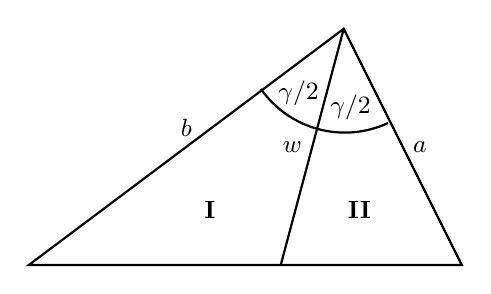
\begin{tikzpicture}
        \coordinate (A) at (-4,0);
        \coordinate (B) at (1.5,0);
        \coordinate (C) at (0,3);
        \draw[thick] (A) -- (B) --node[right]{$a$} (C) --node[above]{$b$} cycle; 
        \draw[thick] (C) --node[left]{$w$} (-0.8,0);
        \draw[thick] ($(C)+(216:1.3)$) arc (215:295:1.3);
        \node (A) at ($(C)+(215+20:1)$){$\gamma/2$};
        \node (A) at ($(C)+(295-20:1)$){$\gamma/2$};
        \node (A) at (-1.7,0.7){\textbf{I}};
        \node (A) at (0.2,0.7){\textbf{II}};
        % \draw[thick] ($(C)+(216:1.6)$) arc (215:255:1.6);
    \end{tikzpicture}
    \vspace{-5mm}
\end{wrapfigure}

\begin{align}
    &\text{Fläche in I:} \quad A_1 = \frac{bw}{2} \sin(\frac{\gamma}{2})\\
    &\text{Fläche in II:} \quad A_2 = \frac{aw}{2} \sin(\frac{\gamma}{2})\\
    &\text{Gesamtfläche:} \quad A = \frac{ab}{2} \sin(\gamma) \\
    &\text{andererseits: } \quad A= A_1 + A_2  \quad \Rightarrow \quad \frac{ab}{2}\cancel{\sin\gamma} = \frac{(a+b)w}{2} \sin(\frac{\gamma}{2}) = \frac{(a+b)w}{4} \frac{\cancel{\sin\gamma}}{\cos(\frac{\gamma}{2})} \\
    &\Rightarrow \cos(\frac{\gamma}{2}) = \frac{(a+b)w}{2ab} \\
    & \Rightarrow A = \frac{(a+b)w}{2} \sin(\frac{\gamma}{2}) =\frac{(a+b)w}{2}\sqrt{1-\cos^2\qty(\frac{\gamma}{2})} = \uuline{\frac{(a+b)w}{2}\sqrt{1-\frac{(a+b)^2 w^2}{4a^2b^2}}}.
\end{align}
\Titelbanner{7}{Grundlagen der Differentialrechnung\\Kurvendiskussion}

\paragraph{Wiederholung Ableitungsregeln}$~$
\begin{itemize}
    \item Linearität: $\dv{x}(a f(x) + b g(x)) = a \dv{f}{x} + b \dv{g}{x}$
    \item Produktregel (Leibniz-Regel): $\dv{x}(f(x)\cdot g(x)) = \dv{f}{x} \cdot g(x) + f(x) \cdot \dv{g}{x}$
    \item Kettenregel: $\dv{x} f(g(x)) = \qty(\dv{f}{g})(g(x))\cdot \dv{g}{x}.$
    % \item Quotientenregel: $\dv{x}\qty(\frac{f(x)}{g(x)}) = \frac{1}{g(x)^2} \qty(\dv{f}{x}\cdot g(x) - f(x) \cdot \dv{g}{x}).$
    \item Potenzregel: $\dv{x}\qty(x^n) = n \, x^{n-1}.$
\end{itemize}
\emph{Ableitungen spezieller Funktionen: }
\begin{alignat}{3}
    \dv{x}\sin(x) &= +\cos(x) &\qquad\quad \dv{x}\exp(x) &= \exp(x)\\
    \dv{x}\cos(x) &= -\sin(x) & \dv{x}a^x &= \ln(a) a^x.
\end{alignat}

\emph{Beispiel:}\\[-1.5cm]
\begin{align}
    f(x) &= x^2 \ln\big(\underbrace{3x^2-5x+2}_{g(x)}\big) \\
    \quad\Rightarrow f'(x) &= 2x \ln(g(x)) + x^2 \frac{1}{g(x)} \dv{g(x)}{x}= 2x \ln(3x^2-5x+2) + \frac{x^2(6x-5)}{3x^2 - 5x+2}.
\end{align}

\paragraph{Aufgabe 1: } \emph{Ableitungen I} \hfill Ziel: (a) bis (e)\\[0.2cm]
\emph{Berechnen Sie die Ableitungen der folgenden Funktionen.}
\begin{enumerate}[label=(\alph*)]
    \setlength{\mathindent}{0cm}
    \item $Q(r)=\frac{3r^2}{2}\qty(\frac{1}{2}+\ln\frac{r}{r_0})$
    \begin{align}
        \dv{Q(r)}{r} &= 3r\qty(\frac{1}{2}+\ln(\frac{r}{r_0})) + \frac{3r^2}{2}\frac{r_0}{r}\frac{1}{r_0} = \uuline{3r\qty(1+\ln \frac{r}{r_0})}.
    \end{align}
    \item $f(x)=\cos^4(3tx)-\sin^4(3tx) = \underbrace{(\cos^2(3tx)+\sin^2(3tx))}_{1}(\cos^2(3tx)-\sin^2(3tx))$ 
    \begin{align}
        \dv{f(x)}{x} = -6t \sin(3tx)\cos(3tx) - 6t\sin(3tx)\cos(3tx) = \uuline{-12t \sin(3tx)\cos(3tx)}.
    \end{align}
    \item $S(\tau)=(\tau-1)\e^{\tau}+\frac{\tau^2}{4}\qty(2\ln\tau-1)$
    \begin{align}
        \dv{S(\tau)}{\tau} = \cancel{\e^{\tau}} + (\tau-\cancel{1})\e^\tau + \frac{\tau}{2}\qty(2\ln(\tau)-\cancel{1}) + \frac{\tau^{\cancel{2}}}{4} \frac{2}{\cancel{\tau}} = \uuline{\tau(\e^{\tau} + \ln(\tau))}.
    \end{align}
    \item $y(x)=\frac{\exp(2x)}{25}\qty[(5x-4)\sin x+(10x-3)\cos x]$
    \begin{align}
        \dv{y(x)}{x} &= \frac{2}{25} \e^{2x} \bigg[\hdots \bigg] + \frac{1}{25}\e^{2x} \qty[5 \sin(x) + (5x-4)\cos(x) + 10\cos(x)-(10x-3)\sin(x)] \\
        &= \frac{\e^{2x}}{25}\qty[\cancel{(10x-8)\sin(x)}+(20x-\bcancel{6})\cos(x) + (5x+\bcancel{6})\cos(x) - \cancel{(10x-8)\sin(x)}] \notag \\
        &= \uuline{x \cos(x) \e^{2x}}
    \end{align}
    \item $F(x)=-\frac{k}{\sqrt{(x-x_0)^2+(y-y_0)^2}}$
    \begin{align}
        \dv{F(x)}{x} &= \frac{k}{\cancel{2}} \frac{\cancel{2}(x-x_0)}{\sqrt{\hdots}^3} = \uuline{\frac{k(x-x_0)}{\sqrt{(x-x_0)^2+(y-y_0)^2}^3}}
    \end{align}
    \item$~$\\[-1.5cm]
    \begin{align}
        N(z) &=\underbrace{\frac{2\cos\qty(\frac{z}{2})}{\sqrt{1+\cos(z)}}}_{\mathclap{1+\cos(z) = 2 \cos^2\qty(\frac{z}{2})}}\qty[\ln\qty(\cos\frac{z}{4}+\sin\frac{z}{4})-\ln\qty(\cos\frac{z}{4}-\sin\frac{z}{4})] \qquad \sigma_{\pm} = \cos(\frac{z}{4})\pm \sin(\frac{z}{4}) \\
        &= \sqrt{2}(\ln(\sigma_+)-\ln(\sigma_-)) \\
        \Rightarrow \dv{N(z)}{z} &= \sqrt{2} \qty(\frac{(\sigma^+)'}{\sigma^+} - \frac{(\sigma^-)'}{\sigma^-}) = \sqrt{2} \frac{(\sigma^+)' \sigma^- - (\sigma^-)'\sigma^+}{\sigma^+ \sigma^-} \qq{mit} (\sigma^\pm)' = \pm \frac{1}{4}\sigma^\mp \\
        &= \frac{1}{2\sqrt{2}} \frac{(\sigma^+)^2 + (\sigma^-)^2}{\sigma^+ \sigma^-} = \frac{1}{\cancel{2}\sqrt{2}} \frac{\cancel{2}}{\cos^2\qty(\frac{z}{4})-\sin^2\qty(\frac{z}{4})} \notag \\
        &= \frac{1}{\sqrt{2}} \frac{1}{2\cos^2\qty(\frac{z}{4}-1)} = \frac{1}{\sqrt{2}} \frac{1}{\cos(\frac{z}{2})} = \uuline{\frac{1}{\sqrt{1+\cos(z)}}}.  
    \end{align}
\end{enumerate}
%
\paragraph{Aufgabe 2: } \emph{Ableitungen II}\hfill Ziel: (a) bis (d)\\[0.2cm]
\emph{Finden Sie die $n$-te Ableitung der folgenden Funktionen.}
    \begin{enumerate}[label=(\alph*)]
        \item $f(x)=x^n$
        \item $f(x)=\e^{kx}+\e^{-kx}$
        \item $f(x)=x^{n-1}$
        \item $f(x)=a^x$ 
        \item $f(x)=\frac{1}{1-x}$
        \item[(f)*] $f(x)=\frac{x}{1-x-x^2}$ 
    \end{enumerate}
%
\paragraph{Aufgabe 3: } \emph{Kurvendiskussion I}\\[0.2cm]
\emph{Ein zweiatomiges Molekül lässt sich näherungsweise durch das sogenannte ``Morse-Potential'' beschreiben,}
\begin{align*}
U(x)=D\qty(\e^{-2\alpha x}-2\e^{-\alpha x})\,, \hspace{1cm} D,\alpha=\operatorname{const}.
\end{align*}
\begin{itemize}
\item Bestimmen Sie Nullstellen und lokale Extrema der Funktion $U(x)$ sowie deren Verhalten für $x \to\pm\infty$.
\item Skizzieren Sie die Funktion $U(x)$ für $D=\alpha=1$ im Intervall $x\in[-1,5]$.
\end{itemize}
%
\paragraph{Aufgabe 4: } \emph{Kurvendiskussion II}\\[0.2cm]
\emph{Die Bewegung eines Teilchens mit Drehimpuls $L$ und Energie $E$ in der gekrümmten Raumzeit eines Schwarzen Loches der Masse $m$ wird beschrieben durch das Potential}
\begin{align*}
U(r)=\frac{E}{2}-\frac{Em}{r}+\frac{L^2}{2r^2}-\frac{mL^2}{r^3}\,, \hspace{1cm} r>0\,.
\end{align*}
\begin{itemize}
\item \emph{Bestimmen Sie Nullstellen und lokale Extrema der Funktion $U(r)$ sowie deren Verhalten für $\to\infty$ und $\to 0$.}
\item \emph{Setzen Sie $\textstyle m=\frac{1}{2}$. Welche Bedingungen an $E$ und $L$ müssen erfüllt sein, damit $U(r)$ zwei, ein oder keine lokalen Extrema besitzt?}
\item \emph{Skizzieren Sie die Funktion $U(r)$ für $E=1$ und $L=2$ (nicht maßstabsgerecht).}
\end{itemize} 
%
\paragraph{Aufgabe 5: } \emph{Gewöhnliche Differentialgleichungen}\hfill (Zusatzaufgabe)\\[0.2cm]
\begin{enumerate}[label=(\alph*)]
\item \emph{Finden Sie eine Funktion $f(x)$, welche die folgende Gleichung erfüllt:}
\begin{align*}
f''(x)=a^2f(x)+bx\,.
\end{align*}
\item \emph{Finden Sie eine Funktion $f(x)$, welche die folgende Gleichung erfüllt:}
\begin{align*}
f'(x)=\qty(1+\ln(x))f(x)\,.
\end{align*}
\end{enumerate}
\Titelbanner{8}{Die Methode der vollständigen Induktion}

\paragraph{Aufgabe 1: } \emph{Rekursive und explizite Zuordnungsvorschrift}\\[0.2cm]
Eine Reihe $(a_n)_{n\in\mathbb{N}_0}$ sei rekursiv definiert durch
\begin{align*}
a_{n+1}=2a_n+1\,, && a_0=0\,.
\end{align*}
Finden Sie einen expliziten Ausdruck für $a_n$ und beweisen Sie ihn per vollständiger Induktion.
%
%
\paragraph{Aufgabe 2: } \emph{Vollständige Induktion I}\\[0.6cm]
Beweisen Sie\\[-1.5cm]
\begin{align*}
S_n&=1^2-2^2+3^2-4^2+\hdots+(-1)^{n-1}n^2=(-1)^{n-1}\,\dfrac{n(n+1)}{2}\,.
\end{align*}
%
\paragraph{Aufgabe 3: } \emph{Vollständige Induktion II}\\[0.2cm]
Beweisen Sie, dass die Summe der Kuben der ersten $n$ natürlichen Zahlen gleich $\left[\frac{n(n+1)}{2}\right]^2$ ist. 
%
\paragraph{Aufgabe 4: } \emph{Vollständige Induktion III}\\[0.2cm]
Zeigen Sie, dass die Summe der Kuben dreier aufeinanderfolgender natürlicher Zahlen durch $9$ teilbar ist.
%
\paragraph{Aufgabe 5: } \emph{Die Suche nach der richtigen Summenformel}\\[0.2cm]
Stellen Sie eine Summenformel für das Polynom
\begin{align*}
S_n = 1-\dfrac{x}{1!}+\dfrac{x(x-1)}{2!}-\hdots+(-1)^n \dfrac{x(x-1)\dots(x-n+1)}{n!}
\end{align*}
auf und beweisen Sie deren Richtigkeit durch vollständige Induktion.
%
\paragraph{Aufgabe 6: } \emph{Fibonacci-Zahlen}\hfill (Zusatzaufgabe)\\[0.2cm]
Die Folge der Fibonacci-Zahlen ist definiert durch $a_{n+1}=a_n+a_{n-1}$ für $n\ge 1$ und die Startwerte $a_0=0$ und $a_1=1$. Beweisen Sie, dass der explizite Ausdruck für die $n$-te Fibonacci-Zahl gegeben ist durch
\begin{align*}
a_n=\frac{1}{\sqrt{5}}\left(x_+^n-x_-^n\right)\,, \qq{mit} x_{\pm}=\frac{1\pm\sqrt{5}}{2}\,.
\end{align*}
\Titelbanner{9}{Arithmetische \& geometrische Reihen\\
                Der binomische Satz}

\paragraph{Aufgabe 1: } \emph{Arithmetische Reihe}

Wiederholung arithmetische Reihe: $\sum_{k=0}^n (a_0 + k \cdot d) = (n+1)\qty(a_0 + n \frac{d}{2})$ 

\emph{Tafelbeispiel:} 
\begin{itemize}
    \item Summe der ersten $n$ durch fünf teilbaren Zahlen 
    \begin{align}
        0 + 5 + 10 +15 + 20 + \hdots = \sum_{k=0}^n (0+k \cdot 5) = \uuline{\frac{5n(n+1)}{2}}.
    \end{align}
    \item Summe der ersten $n$ ungeraden Zahlen 
    \begin{align}
        \sum_{k=0}^n (2k+1) = (n+1)^2 \qquad (a_0 = 1, d=2).
    \end{align}
\end{itemize}

\emph{Eine Spirale bestehe aus zwei Scharen konzentrischer Halbkreise um die Punkte $A$ und $B$. Es sei $r$ der Radius des innersten Halbkreises und die Strecke $\overline{AB}=e$.}
\begin{enumerate}[label=(\alph*)]\setlength{\itemsep}{-0.5ex}
\item \emph{Wie lang ist der $n$-te Halbbogen?}
\item \emph{Wie lang ist der Gesamtbogen der Spirale bis dahin?}
\end{enumerate}
\begin{figure}[htp]
    \centering
    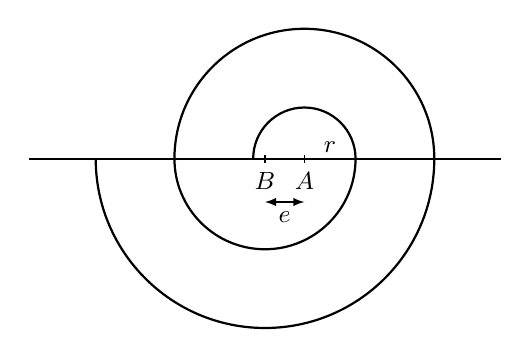
\begin{tikzpicture}[scale=0.5]
        \draw[thick] (-6,0) -- (6,0);
        \draw[thick] (2.3, 0) arc(0:-180:2.3); 
        \draw[thick] (4.3, 0) arc(0:-180:4.3);
        \draw (0,-.1)node[below]{$B$} -- (0,.1); 
        \draw[{latex}-{latex}] (0,-1.1) --node[below]{$e$} (1,-1.1);
        \begin{scope}[shift={(1,0)}]
            \node (A) at (0.65,0.3){$r$};
            \draw (0,-.1)node[below]{$A$} -- (0,.1);
            \draw[thick] (1.3, 0) arc(0:180:1.3); 
            \draw[thick] (3.3, 0) arc(0:180:3.3); 
        \end{scope}
    \end{tikzpicture}
    \vspace{-1.5cm}
\end{figure}

\emph{Lösung:}
\begin{align}
    \begin{rcases}
        \text{1. Halbbogen: } & L_1 = \pi r \\
        \text{2. Halbbogen: } & L_2 = \pi (r+e) \\
        \text{3. Halbbogen: } & L_3 = \pi (r+2e) \\
    \end{rcases} \quad \text{n. Halbbogen:}\quad L_n = \pi r + \pi e (n-1) 
\end{align}
Die Länge der Spirale bis zum $n$-ten Halbbogen: 
\begin{align}
    S_n = \sum_{k=1}^n L_k = n\pi r + \pi e \underbrace{\sum_{k=1}^n k}_{\frac{n\cdot(n+1)}{2}} - n \pi e = n\pi \qty(r + e \frac{n-1}{2}). 
\end{align}
%
\paragraph{Aufgabe 2: } \emph{Geometrische Folge}\\[0.2cm]
\emph{Beim Durchgang durch eine Glasplatte verliert ein Lichtstrahl $\textstyle\frac{1}{12}$ seiner Lichtstärke. Wie viele Platten muss er durchdringen, wenn er nur noch die Hälfte der ursprünglichen Lichtstärke besitzen soll?}\\[0.2cm]
\emph{Hinweis:} \emph{Es genügt die Angabe des Ergebnisses in impliziter Form.}
\begin{itemize}
    \item Lichtstärke nach einem Durchgang: $I_1 = \frac{11}{12} I_0$
    \item Lichtstärke nach $n$ Durchgängen: $I_n = \qty(\frac{11}{12})^n L_0 \overset{!}{=} \frac{1}{2} L_0$
\end{itemize}
\begin{align}
    \Rightarrow \quad n = \frac{\ln(1/2)}{\ln(11/12)} \approx 7.97.
\end{align}
Es müssen also 8 Platten durchdrungen werden, damit der Lichtstrahl auf die Hälfte der Intensität abfällt.
%
\paragraph{Aufgabe 3: } \emph{Geometrische Reihe}

Wiederholung geometrische Reihe: $a_0 \sum_{k=0}^n q^k = a_0\frac{1-q^{n+1}}{1-q}$.
\begin{align}
    \text{Beispiel:} \qquad \sum_{k=0}^n \e^{kx} = \sum_{k=0}^n (\e^x)^k = \uuline{\frac{1-(\e^{x})^{n+1}}{1-\e^{x}}}.
\end{align}

\emph{Es sei eine Anordnung aus zwei Glasplatten gegeben, in die ein Laserstrahl der Intensität $I_\text{in}$ eingeschossen werde. Jede Platte besitze einen Transmissionskoeffizienten $T$ ($0<T<1$), d.h. dass an jeder Platte von einem Lichtstrahl der Intensität $I$ ein Anteil $T\cdot I$ transmittiert und ein Anteil $(1-T)I$ reflektiert wird.
Bestimmen Sie die Intensität $I_\text{out}$, mit der das Licht auf der anderen Seite der Anordnung austritt.}\\
\begin{center}
    \vspace{-1cm}
\begin{tikzpicture}[scale=0.8]
    \node [] at(0.2,0){$I_\text{out}$};
    \draw [<-,line width=0.8pt] (0.7,0)--(2.7,0);
    \draw [line width=1pt] (3.0,-2)--(3.0,2);
    \draw [line width=1pt] (6.0,-2)--(6.0,2);
    \draw [<-,line width=0.8pt] (3.3,0.15)--(5.7,0.15);
    \draw [->,line width=0.8pt] (3.3,-0.15)--(5.7,-0.15);
    \draw [<-,line width=0.8pt] (6.3,0)--(8.3,0);
    \node [] at(8.8,0){$I_\text{in}$};
    \node [below] at(3,-2){$T$};
    \node [below] at(6,-2){$T$};
\end{tikzpicture}
% \vspace{-2cm}
\end{center}
Die Intensität nach $n$-maligem Hinundherlaufen zwischen den Glasplatten (nur austretender Anteil) ergibt sich 
\begin{align}
    \begin{rcases}
        I_0 = T^2 I_\text{in} \\
        I_1 = T^2 (1-T)^2 I_\text{in} \\
        I_2 = T^2 (1-T)^4 I_\text{in}
    \end{rcases} \qquad I_n = T^2 (1-T)^{2n} I_n. 
\end{align}
Die Gesamtintensität am Ausgang ergibt sich aus der Summe der Teilintensitäten: 
\begin{align}
    I_\text{out} &= \sum_{n=0}^\infty I_\text{in} = T^2 I_\text{in} \sum_{n=0}^\infty (1-T)^{2n} \notag \\
    &= T^2 I_\text{in} \lim_{k\to \infty} \sum_{n=0}^k \qty[(1-T)^2]^n = T^2 I_\text{in} \lim_{k\to \infty} \frac{1-\qty[(1-T)^2]^{k+1}}{1-(1-T)^2} \\
    &= T^2 I_\text{in} \frac{1}{1-(1-T)^2} =  \frac{T^2}{2T - T^2} I_\text{in}= \uuline{\frac{T}{2 - T} I_\text{in}}.
\end{align}

\paragraph{Aufgabe 4: } \emph{Der binomische Satz}

\begin{mymathbox}[ams align, title={Binomialkoeffizenten, binomischer Satz}, colframe={FSUblau}]
    \binom{n}{k} &= \frac{n!}{k!(n-k)!} \qq{,} \binom{n}{k} = \binom{n}{n-k} \qq{für} k \le n\\
    (a+b)^n &= \sum_{k=0}^n \binom{n}{k} a^{n-k} b^k \qq{für} a,b \in \mathbb{R}, n\in\mathbb{N}_0
    \end{mymathbox}


\begin{enumerate}[label=(\alph*)]
\item \emph{Berechnen Sie $(1+a)^6+(1-a)^6$}.
Zeichnen wir dazu das Pascal'sche Dreieck 
\begin{figure}[htp]
    \centering
    \begin{tikzpicture}[scale=0.7]
        \foreach{\x} in {0,...,6}{
            \foreach{\y} in {\x,...,6}{
                \pgfmathsetmacro{\binomial}{int(round(factorial(\y)/(factorial(\x)*factorial(\y-\x))))}
            \node at (2*\x-\y,-\y) {$\binomial$};
            } 
        }
        \draw[thick, red, -{latex}] ($(0,-2)+(-.2,-.2)$) -- +(-.6,-.6);
        \draw[thick, red, -{latex}] ($(-2,-2)+(.2,-.2)$) -- +(.6,-.6);
        \draw[thick, PAForange, -{latex}] (-8,-6)node[left]{$n=6$} -- (-6.5,-6);
    \end{tikzpicture}
\end{figure}
Bei der Summe der beiden Terme fallen nun die ungeraden Potenzen von $a$ weg, während die geraden doppelt auftreten.
\begin{align}
    (1\pm a)^6 &= 1 \pm 6a + 15a^2 \pm 20a^3 + 15a^4 \pm 6a^5 + a^6 \\
    \Rightarrow (1+a)^6 + (1-a)^6 &= 2 + 30a^2 + 30 a^4 + 2 a^6.
\end{align}
\item \emph{Schreiben Sie die allgemeine Binomialformel für $(1+x)^n$ und $(1-x)^n$ auf und setzen Sie anschließend $x=1$. In letzterem Falle sei $n\ge 1$.}
\begin{alignat}{3}
    (1+x)^n &= \sum_{k=0}^n \binom{n}{k} x^k \qquad &&\overset{x=1}{\Longrightarrow} \quad \uuline{\sum_{k=0}^n \binom{n}{k} = 2^n} \\
    (1-x)^n &= \sum_{k=0}^n (-1) \binom{n}{k} x^k \qquad &&\overset{x=1}{\Longrightarrow} \quad \uuline{\sum_{k=0}^n (-1)^k\binom{n}{k} = 0}.
\end{alignat}
Das sind nützliche Identitäten im Umgang mit Binomialkoeffizienten. Man veranschauliche sich die Ausdrücke im Pascal'schen Dreieck.
\item \emph{Es seien die Funktionen $f(x)=\left(\e^{x}+\e^{-x}\right)/2$ und $g(x)=\left(\e^{x}-\e^{-x}\right)/2$ definiert. Finden Sie einen Ausdruck, der $f(nx)+g(nx)$, mit $n\in\mathbb{N}$, auf (Potenzen von) $f(x)$ und $g(x)$ zurückführt.}
\begin{align}
    &\begin{rcases}
        f(x) = \frac{1}{2}(\e^{x}+\e^{-x}) \\
        g(x) = \frac{1}{2}(\e^{x}+\e^{-x})
    \end{rcases} \quad \e^{x} = f(x) + g(x) \\
    &\Rightarrow f(nx) + g(nx) = \e^{nx} = (f(x) + g(x))^n = \uuline{\sum_{k=0}^n \binom{n}{k} f(x)^k g(x)^{n-k}}.
\end{align}
Das ist die Formel von Moivre für Hyperbolikus-Funktionen.
\end{enumerate}
%
\paragraph{Aufgabe 5: } \emph{Erzeugende Funktion} \hfill (Zusatzaufgabe)\\[0.2cm]
\emph{Betrachten Sie die Rekursionsgleichung $a_{n+1}=2a_n+1$ mit Anfangswert $a_0=0$ aus Aufgabe 1, Thema 8. Es sei eine (unbekannte) Funktion definiert als}
\begin{align*}
f(x)=\sum\limits_{n=0}^\infty a_n x^n\,.
\end{align*}
\begin{enumerate}[label=(\alph*)]
\item \emph{Multiplizieren Sie beide Seiten der Rekursionsgleichung mit $x^n$, summieren Sie über $n$ (von Null bis Unendlich) ab und versuchen Sie alle auftretenden Terme durch $f(x)$ auszudrücken. Lösen Sie für $f(x)$.}
\begin{align}
    a_{n+1} x^n &= 2 a_n x^n + x^n \\
    \Rightarrow \sum_{n=0}^\infty &= 2 \underbrace{\sum_{n=0}^\infty a_n x^n}_{f(x)} + \underbrace{\sum_{n=0}^\infty x^n}_{\mathrlap{\hspace{-0.3cm}\frac{1}{1-x}, \qq{geometrische Reihe}}} \\
    \Rightarrow \underbrace{\sum_{n=1}^\infty a_n x^{n-1}} &= 2 f(x) + \frac{1}{1-x} \\
    \sum_{n=0}^\infty a_n &x^{n-1} - \cancel{a_0 x^{-1}} = \frac{1}{x} \sum_{n=0}^\infty a_n x^n = \frac{1}{x} f(x) \\
    \Rightarrow f(x) &= 2x f(x) + \frac{x}{1-x} \quad \Rightarrow \quad f(x) = \frac{x}{(1-x)(1-2x)}.
\end{align}
\item \emph{Nutzen Sie Ihr Wissen über geometrische Reihen, um $f(x)$ wieder in Reihendarstellung zu überführen und lesen Sie die Koeffizienten vor $x^n$ ab.}
\begin{align}
    f(x) &= x \underbrace{\frac{1}{(1-x)(1-2x)}}_{\mathclap{\text{Partialbruchzerlegung}}} = x \qty(\frac{\alpha}{1-2x} + \frac{\beta}{1-x})= x \qty(\frac{2}{1-2x}-\frac{1}{1-x}).   \\
    &\quad 1 = \alpha(1-x)+\beta(1-2x) = -x(\alpha+2\beta) + (\alpha+\beta) \\
    &\quad 1 = \alpha + \beta \qq{und} 0 =\alpha + 2\beta  \qquad \Rightarrow \quad \alpha = 2, \beta = -1.
\end{align}
Nun nutzen wir die Ausdrücke für die geometrische Reihe 
\begin{align}
    \frac{1}{1-x} &= \sum_{n=0}^\infty x^n \qq{,} \frac{1}{1-2x} = \sum_{n=0}^\infty (2x)^n \\
    \Rightarrow f(x) &= x(2 \sum_{n=0}^\infty 2^n x^n - \sum_{n=0}^\infty x^n) = x \sum_{n=0}^\infty (2^{n+1} - 1) x^n \\
    &= \sum_{n=1}^\infty (2^n -1) x^n \quad \Rightarrow \quad \uuline{a_n = 2^n -1}.
\end{align}
\end{enumerate}
%
% \paragraph{Aufgabe 6*: } \emph{Zustandssumme}\\[0.2cm]
% Vereinfachen Sie den Ausdruck
% \begin{align*}
% \Omega_N=\sum\limits_{n_1=0}^N\sum\limits_{n_2=0}^N\sum\limits_{n_3=0}^N\dots\sum\limits_{n_k=0}^N f(n_1)f(n_2)f(n_3)\dots f(n_k)\,, \qq{wobei}f(n)=\e^{-n}.
% \end{align*}
% Bestimmen Sie anschließend den Grenzwert $\Omega=\lim\limits_{N\rightarrow\infty}(\Omega_N)$.
% %
% \paragraph{Aufgabe 7*: } \emph{Fibonacci-Zahlen II}\\[0.2cm]
% Wenden Sie das Verfahren aus Aufgabe 5 auf die Folge $a_{n+1}=a_n+a_{n-1}$ der Fibonacci-Zahlen mit Startwerten $a_0=0$, $a_1=1$ an. Beachten Sie, dass hier $n\ge 1$ gelten muss.
%
\Titelbanner{10}{Integralrechnung}

\paragraph{Wiederholung Integralrechnung}$~$

\begin{itemize}
    \item Integrale von Polynomen: $\int \dd{x} (x^3+5x^2+1) = \frac{x^4}{4}+\frac{5x^3}{3} + x + C.$ 
    \item Logarithmische Integration: $\int \dd{x} \frac{2x+3}{x^2+3x+19} = \ln|x^2+3x+19| + C$ 
    \item Integrale mit Wurzeln: $\int \dd{x} \frac{1}{\sqrt{x}} = 2\sqrt{x} + C$
    \item Partielle Integration: $\int\limits_{a}^{b} \dd{x} u'(x) v(x) = u(x) v(x)\eval_a^b - \int\limits_{a}^{b}\dd{x} u(x) v'(x)$
\end{itemize}

\emph{Tafelbeispiel:}
\begin{align}
    \int \dd{x} \underbrace{x^n}_{u'} \underbrace{\ln(x)}_{v} &= \frac{x^{n+1}}{n+1} \ln(x) - \int \dd{x} \frac{x^{n+\cancel{1}}}{n+1}\cdot \frac{1}{x} \quad (n\neq -1) \\
    &= \frac{x^{n+1}}{n+1} - \frac{x^{n+1}}{(n+1)^2} + C= \uuline{\frac{x^{n+1}}{(n+1)^2}((n+1)\ln(x)-1) + C}
\end{align}

\paragraph{Aufgabe 1: } \emph{Stammfunktionen} \hfill Ziel: (a) bis (d)\\[0.2cm]
\emph{Bestimmen Sie jeweils die Stammfunktion $F(x)$ der folgenden Funktionen.}
\emph{Hinweis: Partialbruchzerlegung in (e).}\\[1cm]

\begin{enumerate}[label=(\alph*)]
    \setlength{\mathindent}{0pt}
    \item$~$\\[-1.5cm] 
    \begin{align}
        f(x)=\sin(2x+5) \quad \Rightarrow \quad F(x) = \int \dd{x} \sin(2x+5) = \uuline{-\frac{\cos(2x+5)}{2}+C}.
    \end{align}
    \item$~$\\[-1.5cm]
    \begin{align}
        f(x)=\frac{k}{kx+1} \quad \Rightarrow \quad F(x) = k \int \dd{x} \frac{1}{kx+1} = \uuline{\ln|kx+1| + C}
    \end{align}
    \item$~$\\[-1.5cm] 
    \begin{align}
        f(x)=\frac{\cos(x)}{\sin(x)} \quad \Rightarrow \quad F(x) = \int \dd{x} \frac{\cos(x)}{\sin(x)} = \uuline{\ln(\sin(x))+C}
    \end{align}
    \item $f(x)=\frac{a\cos(x)+b\sin(x)}{c\sin(x)} = \frac{a}{c}\frac{\cos(x)}{\sin(x)} + \frac{b}{c}$
    \begin{align}
        F(x) = \frac{a}{c} \int\dd{x} \frac{\cos(x)}{\sin(x)} + \frac{b}{c} \int \dd{x} = \uuline{\frac{a \ln(\sin(x))+bx}{c}+ C}  
    \end{align}
    \item$~$\\[-1.5cm] 
    \begin{align}
        f(x)=\frac{x^2+1}{x^2-1} &= \alpha + \frac{\beta}{x+1} + \frac{\gamma}{x-1}  \\
        \Rightarrow x^2 + 1 &= \alpha (x^2-1) + \beta (x-1) + \gamma (x+1) = \underbrace{\alpha}_{=1} x^2 + \underbrace{(\beta+\gamma)}_{=0} x + \underbrace{(\gamma - \beta -\alpha)}_{=1} \\[-5mm]
        \frac{x^2+1}{x^2-1} &= 1 - \frac{1}{x+1} + \frac{1}{x-1} \\
        F(x) &= \int\dd{x} - \int\frac{\dd{x}}{x+1} + \int \frac{\dd{x}}{x-1} = \uuline{x + \ln(\frac{x-1}{x+1})+C} 
    \end{align}
    \item$~$\\[-1.5cm]  
    \begin{align}
        f(x)=\frac{kx}{\sqrt{x^2+y^2}^3} \quad \Rightarrow \quad F(x) = k \int \frac{x}{\sqrt{x^2+y^2}^3} \dd{x} = \uuline{- \frac{k}{\sqrt{x^2+y^2}} + C}.
    \end{align}
\end{enumerate}
%
\paragraph{Aufgabe 2: } \emph{Partielle Integration}\hfill Ziel: (a) bis (c)\\[0.2cm]
\emph{Bestimmen Sie die folgenden Integrale unter Verwendung partieller Integration.}

\begin{enumerate}[label=(\alph*)]
    \setlength{\mathindent}{0pt}
    \item$~$\\[-1.7cm]
    \begin{align}
        \int\limits_0^\pi \underbrace{x}_{u}\underbrace{\sin(x)}_{v'}\dd{x} = \qty(-x \cos(x))\eval_0^\pi + \int\limits_{0}^{\pi} \cos(x) \dd{x} = \pi + \sin\eval_0^\pi = \uuline{\pi}
    \end{align}
    \item$~$\\[-1.7cm]
    \begin{align}
        \int\limits_0^1 \underbrace{x^3}_{u}\underbrace{\e^{x}}_{v'}\dd{x} &= x^3 \e^x \eval_0^1 - 3 \int\limits_{0}^{1} x^2 \e^x \dd{x} = \e - 3(x^2 \e^x)\eval_0^1 + 6 \int\limits_{0}^{1}x\e^x \dd{x} \\
        &= -2\e + \cancel{6(x\e^x)\eval_0^1} - 6 \underbrace{\int\limits_{0}^{1}\e^x \dd{x}}_{\cancel{\e}-1} = \uuline{6-2\e}.
    \end{align}
    \item$~$\\[-1.7cm]
    \begin{align}
        \int\limits_{r_0}^{2r_0} \underbrace{r\vphantom{\qty(\frac{1}{1})}}_{u'}\underbrace{\qty(1+\ln \frac{r}{r_0})}_{v} \dd{r} &= \eval[\frac{r^2}{2}\qty(1+\ln \frac{r}{r_0})|_{r_0}^{2r_0} - \frac{1}{2} \int\limits_{r_0}^{2r_0} r^{\cancel{2}} \cdot \frac{1}{\cancel{r}} \dd{r} \\
        &= 2 r_0^2 (1+\ln2) - \frac{r_0^2}{2} - \frac{1}{4}(4r_0^2 -r_0^2) = \uuline{\qty(\frac{3}{4}+2\ln2)r_0^2}
    \end{align}
    \item$~$\\[-1.5cm]
    \begin{align}
        \underbrace{\int \frac{\ln(x)}{x}\dd{x}}_{\mathclap{u'= \frac{1}{x}, v=\ln(x)}} = \ln^2(x) - \int \frac{\ln(x)}{x} \quad \Rightarrow \int \frac{\ln(x)}{x}\dd{x} = \uuline{\frac{\ln^2(x)}{2} + C}.
    \end{align}
\end{enumerate}

\paragraph{Aufgabe 3: } \emph{Substitutionen}\\[0.2cm]
\emph{Berechnen Sie die folgenden Integrale jeweils unter Verwendung der angegebenen Substitution.}

\emph{Tafelbeispiel:}
\begin{align}
    \int \dd{x} \ln(x) &= \int \dd{u} u \e^{(n+1)u} \overset{\text{P.I.}}{=} \frac{u \e^{(n+1)u}}{n+1} - \underbrace{\int \dd{u} \frac{\e^{(n+1)u}}{n+1}}_{\displaystyle\frac{\e^{(n+1)u}}{(n+1)^2}}= \uuline{\frac{x^{n+1} \ln(x)}{n+1} - \frac{x^{n+1}}{(n+1)^2}} \\[-8mm]
    \text{Subst. } u&= \ln(x), \quad \dd{x} = \e^u \dd{u} 
\end{align}
\emph{Lösung:}
\begin{enumerate}[label=(\alph*)]
    \setlength{\mathindent}{0pt}
    \item$~$\\[-1.7cm]
    \begin{align}
        \int\limits_{0}^{1} \sqrt{1-x^2} \dd{x} &= \int\limits_{0}^{\pi/2} \dd{\varphi} \cos(\varphi) \sqrt{1-\sin^2(\varphi)} = \int\limits_{0}^{\pi/2} \dd{\varphi} = \int\limits_{0}^{\pi/2}\dd{\varphi} \frac{1+\cos(2\varphi)}{2} \notag \\
        &\qquad x = \sin\varphi,\quad \dd{x} = \cos\varphi \dd{\varphi}, \qq{Grenzen} x=0: \varphi=0, \quad x=1: \varphi = \frac{\pi}{2} \\
        &= \eval[\frac{\varphi}{2} + \frac{\sin(2\varphi)}{4}|_0^{\pi/2} = \uuline{\frac{\pi}{4}}
    \end{align}
    \item$~$\\[-1.7cm]
    \begin{align}
        \int\limits_0^1 \frac{\dd{x}}{(1+x^2)\sqrt{\arctan(x)}} &= \int\limits_{0}^{\pi/4} \frac{\dd{u}}{\sqrt{u}} = 2 \sqrt{u} \eval_0^{\frac{\pi}{4}} = \uuline{\sqrt{\pi}} \\
        u = \arctan(x), \quad \dd{u} &= \frac{\dd{x}}{1+x^2}, \qq{Grenzen} x=0: u=0, \quad x=1: u=\frac{\pi}{4}
    \end{align}
\end{enumerate}

\paragraph{Aufgabe 4: } \emph{Vollständige Induktion} \hfill (Zusatzaufgabe)\\[0.2cm]
\emph{Zeigen Sie mithilfe vollständiger Induktion, dass für die Fakultät}
\begin{align*}
    n! = \int\limits_{0}^{\infty} x^n \e^{-x} \dd{x},
\end{align*}
\emph{gilt. Hinweis: Es gilt $0! = 1$.}
\begin{enumerate}
    \setlength{\mathindent}{0cm}
    \item[(IA)] $n=0: \quad 0! = \int\limits_{0}^{\infty} \e^{-x} \dd{x} = -\e^{-x}\eval_0^\infty = -(0-1) = 1 \quad\checkmark$ 
    \item[(IV)] $n=k: \quad k! = \int\limits_{0}^{\infty} x^k \e^{-x} \dd{x}$
    \item[(IB)] $n=k+1: \quad (k+1)! = \int\limits_{0}^{\infty} x^{k+1} \e^{-x} \dd{x}$\\
    \begin{proof}$~$\\[-1.8cm]
        \begin{align}
            \hspace{1.5cm} \int\limits_{0}^{\infty} x^{(k+1)} \e^{-x} \dd{x} \overset{\text{P.I.}}{=} \underbrace{\eval(-x^{k+1} \e^{-x}|_0^\infty}_{=0} + (k+1) \underbrace{\int\limits_{0}^{\infty} x^k \e^{-x} \dd{x}}_{k!} = (k+1)k! = (k+1)!
        \end{align}
    \end{proof}
\end{enumerate}

\paragraph{Aufgabe 5: } \emph{Flächenintegral}\\[0.2cm]

\emph{Tafelbeispiel:} Eingeschlossene Fläche einer Parabel $y(x) = 1-x^2$ mit der $x$-Achse. 
\begin{align}
        A = \int\limits_{-1}^{1} \dd{x} \int\limits_{0}^{y(x)}\dd{y} = \int\limits_{-1}^{1}\dd{x} \int\limits_{0}^{1-x^2} \dd{y} = \int\limits_{-1}^{1}\dd{x} (1-x^2) = \eval(x-\frac{x^3}{3}|_{-1}^1 = \frac{4}{3}.
\end{align}
\emph{Leiten Sie die Formel für den Flächeninhalt eines Kreises vom Radius $R$ her.}
\begin{center}
    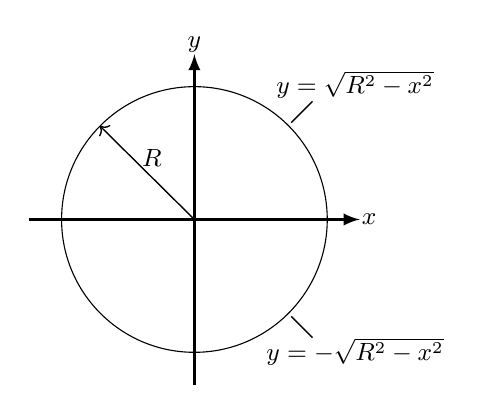
\begin{tikzpicture}[scale=0.6]
        \draw[-{latex}, line width=1pt] (0,-3.5)--(0,3.5);
        \draw[-{latex}, line width=1pt] (-3.5,0)--(3.5,0);
        \draw (0,0) circle (80pt);
        \node at (0,3.7) {$y$};
        \node at (3.7,0) {$x$};
        \draw[line width=0.5pt] (2.05,2.05)--(2.5,2.5);
        \draw[line width=0.5pt] (2.05,-2.05)--(2.5,-2.5);
        \node at (3.4,2.85) {$y=\sqrt{R^2-x^2}$};
        \node at (3.4,-2.8) {$y=-\sqrt{R^2-x^2}$};
        \draw[->,line width=0.5pt] (0,0)--(-2,1.98);
        \node at (-0.9,1.3) {$R$};
    \end{tikzpicture}
\end{center}
\vspace{-1cm}
\begin{align}
    \frac{A}{4} &= \int\limits_{0}^{R} \dd{x} \int\limits_{0}^{\sqrt{R^2-x^2}}\dd{y} = \int\limits_{0}^{R} \dd{x} \sqrt{R^2-x^2} = R \int\limits_{0}^{R}\dd{x} \sqrt{1-\frac{x^2}{R^2}} \qq{Subst.} z = \frac{x}{R} \\
    &= R^2 \int\limits_{0}^{1} \dd{z} \sqrt{1-z^2} \overset{(3a)}{=} \frac{\pi R^2}{4} \quad \Rightarrow \uuline{A = \pi R^2}
\end{align}
% \vspace{1cm}
%
\paragraph{Aufgabe 6: } \emph{Volumenintegral} \hfill (Zusatzaufgabe)\\[0.2cm]
\emph{Berechnen Sie das Volumen des in der Abbildung gezeigten Körpers.}
% \begin{center}
% \includegraphics[width=8cm]{koerper.pdf}
% \end{center}

\begin{figure}[htp]
    \centering
    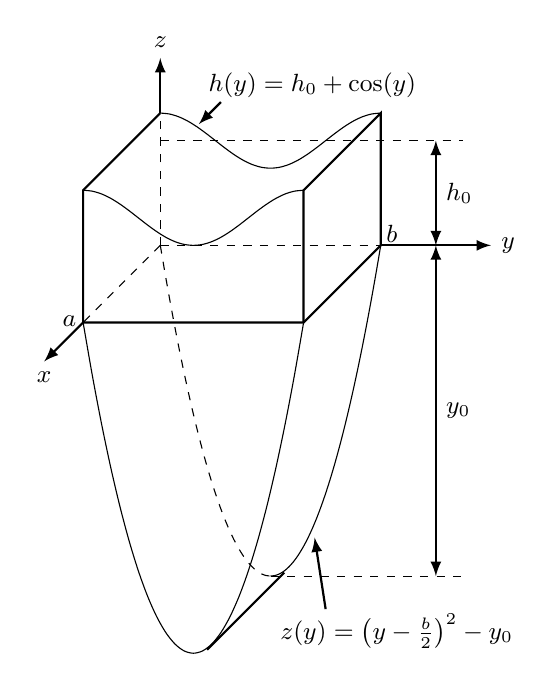
\begin{tikzpicture}[scale=0.7]
        \draw[dashed] (0,0) -- (-1.4,-1.4);
        \draw[dashed] (0,0) -- (0,2.4);
        \draw[dashed] (0,0) -- (4,0);
        \draw[thick,-{latex}] (-1.4,-1.4) -- +(-0.707,-0.707)node[below]{$x$};
        \draw[thick,-{latex}] (4,0) -- +(2,0)node[right]{$y$};
        \draw[thick,-{latex}] (0,2.4) -- +(0,1)node[above]{$z$};
        \draw[thick] (2+0.25,-6+0.0625) -- +(-1.4,-1.4);
        \draw[thick] (-1.4,-1.4) -- ++(4,0) -- ++(1.4,1.4);
        \draw[dashed] (0,1.9) -- +(5.5,0);
        \draw[dashed] (2,-6) -- +(3.5,0);
        \draw[thick, {latex}-{latex}] (5,1.9) --node[right]{$h_0$} (5,0);
        \draw[thick, {latex}-{latex}] (5,0) --node[right]{$y_0$} (5,-6);
        \node (A) at (-1.4-.25,-1.38){$a$};
        \node (A) at (4.2,0.2){$b$};
        \draw[ domain=2:4, smooth, variable=\x] plot ({\x}, {1.5*(\x-2)*(\x-2)-6});
        \draw[ domain=0:2, dashed, smooth, variable=\x] plot ({\x}, {1.5*(\x-2)*(\x-2)-6});
        \draw[ domain=-1.4:2.6, smooth, variable=\x] plot ({\x}, {1.5*(\x-0.6)*(\x-0.6)-6-1.4});
        \draw[ domain=-1.4:2.6, smooth, variable=\x] plot ({\x}, {0.5*cos(deg((\x+1.4)*3.1415/2))+0.5});
        \draw[ domain=0:4, smooth, variable=\x] plot ({\x}, {0.5*cos(deg((\x)*3.1415/2))+0.5+1.4});
        \draw[thick] (-1.4,-1.4) -- ++(0,2.4) -- ++(1.4,1.4);
        \draw[thick] (2.6,-1.4) -- ++(0,2.4) -- ++(1.4,1.4) -- ++(0,-2.4);
        \node[anchor=west] at (0.7,2.9){$h(y)=h_0 + \cos(y) $};
        \draw[thick, -{latex}] (1.1,2.6) --+(-0.4,-.4);
        \node[anchor=west] at (2,-7){$z(y) = \qty(y-\frac{b}{2})^2 - y_0 $};
        \draw[thick, -{latex}] (3,-6.6) --+(-.2,1.3);
    \end{tikzpicture}
\end{figure}

\begin{align}
    V = \int\limits_{0}^{a}\dd{x} \int\limits_{0}^{b}\dd{y} \int\limits_{\qty(y-\frac{b}{2})^2 - y_0}^{h_0 + \cos(y)} \dd{z} &= a \int\limits_{0}^{b} \dd{y} (h_0 + \cos(y) - y^2 - \frac{b^2}{4} + by + y_0) \\
&= ab\qty(h_0 + y_0 - \frac{b^2}{4}) + a \underbrace{\int\limits_{0}^{b}\dd{y} (\cos(y)-y^2 + by)}_{\displaystyle \Bigg(\sin(y) - \frac{y^3}{3} + \frac{by^2}{2}\eval_0^b} \\
&= \uuline{ab\qty(h_0 + y_0 - \frac{b^2}{12})+ a\sin(b)}
\end{align}

\end{document}